\vspace*{-2.0cm}
\textbf{\Huge Results - Easy environment (1) }
\vspace{1.5cm}
\begin{tikzpicture}[remember picture,overlay]
   \node[anchor=south east,inner sep=20pt] at (current page.south east)
              {\includegraphics[scale=0.1]{chapters/res/generated_graph_legend.png}};
\end{tikzpicture}

\begin{figure}[H]
\vspace*{-1cm}
	\makebox[\linewidth][c]{%
	\begin{subfigure}[b]{0.7\textwidth}
		\centering
		\resizebox{0.9\linewidth}{!}{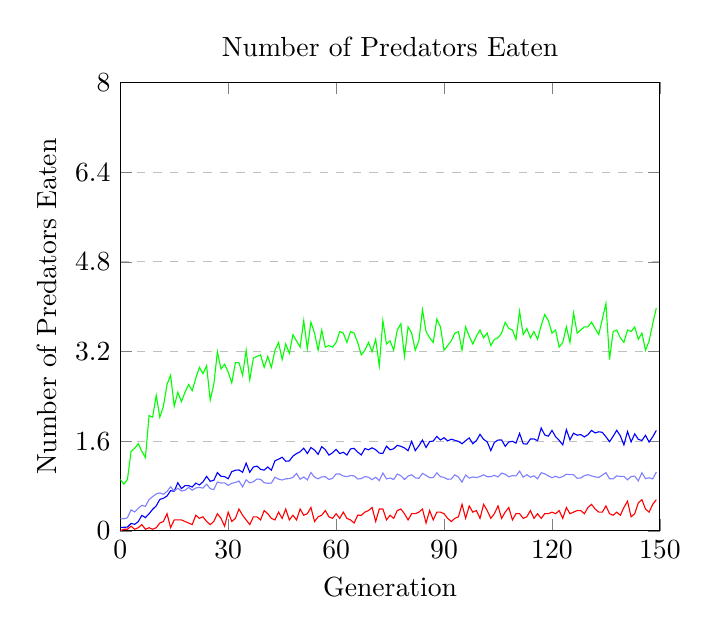
\begin{tikzpicture}
\begin{axis}[
	title={Number of Predators Eaten},
	xlabel={Generation},
	ylabel={Number of Predators Eaten},
	xmin=0, xmax=150,
	ymin=0, ymax=8,
	xtick={0.0,30.0,60.0,90.0,120.0,150.0},
	ytick={0.0,1.6,3.2,4.800000000000001,6.4,8.0},
	ymajorgrids=true,
	grid style=dashed,
]

\addplot[
	color=green,
	]
	coordinates {
	(0,0.9166666666666667)(1,0.8333333333333335)(2,0.9166666666666667)(3,1.4166666666666665)(4,1.4722222222222223)(5,1.5555555555555556)(6,1.4166666666666667)(7,1.3055555555555554)(8,2.0555555555555554)(9,2.027777777777778)(10,2.4166666666666665)(11,2.0277777777777777)(12,2.2222222222222223)(13,2.611111111111111)(14,2.777777777777778)(15,2.222222222222222)(16,2.4722222222222223)(17,2.305555555555556)(18,2.4722222222222223)(19,2.611111111111111)(20,2.5)(21,2.7222222222222228)(22,2.916666666666667)(23,2.8055555555555554)(24,2.944444444444444)(25,2.333333333333333)(26,2.611111111111111)(27,3.194444444444444)(28,2.888888888888889)(29,2.9722222222222228)(30,2.833333333333333)(31,2.6388888888888884)(32,3.0)(33,3.0)(34,2.7777777777777777)(35,3.2222222222222223)(36,2.694444444444444)(37,3.083333333333334)(38,3.1111111111111107)(39,3.138888888888889)(40,2.9166666666666665)(41,3.1111111111111107)(42,2.9166666666666665)(43,3.2222222222222223)(44,3.361111111111111)(45,3.055555555555556)(46,3.3333333333333335)(47,3.166666666666666)(48,3.5)(49,3.3888888888888893)(50,3.2777777777777777)(51,3.75)(52,3.2500000000000004)(53,3.722222222222222)(54,3.527777777777778)(55,3.2222222222222223)(56,3.583333333333333)(57,3.2777777777777786)(58,3.3055555555555554)(59,3.277777777777778)(60,3.3611111111111116)(61,3.5555555555555554)(62,3.5277777777777777)(63,3.361111111111111)(64,3.555555555555556)(65,3.5277777777777777)(66,3.3611111111111107)(67,3.138888888888889)(68,3.222222222222222)(69,3.361111111111111)(70,3.194444444444444)(71,3.4166666666666665)(72,2.944444444444444)(73,3.7500000000000004)(74,3.333333333333333)(75,3.388888888888889)(76,3.2222222222222214)(77,3.583333333333333)(78,3.6944444444444446)(79,3.111111111111111)(80,3.638888888888889)(81,3.5277777777777777)(82,3.2222222222222223)(83,3.388888888888889)(84,3.944444444444444)(85,3.5555555555555554)(86,3.444444444444444)(87,3.361111111111111)(88,3.7777777777777772)(89,3.6388888888888893)(90,3.222222222222222)(91,3.3055555555555554)(92,3.388888888888889)(93,3.5277777777777777)(94,3.5555555555555554)(95,3.222222222222222)(96,3.638888888888889)(97,3.4722222222222223)(98,3.333333333333333)(99,3.4722222222222228)(100,3.5833333333333335)(101,3.444444444444445)(102,3.527777777777778)(103,3.305555555555556)(104,3.4166666666666665)(105,3.4444444444444446)(106,3.5277777777777772)(107,3.722222222222222)(108,3.611111111111111)(109,3.5833333333333335)(110,3.416666666666667)(111,3.9166666666666665)(112,3.5000000000000004)(113,3.611111111111111)(114,3.4444444444444446)(115,3.5555555555555554)(116,3.4166666666666665)(117,3.666666666666667)(118,3.8611111111111107)(119,3.75)(120,3.5277777777777777)(121,3.5833333333333335)(122,3.2777777777777777)(123,3.3611111111111107)(124,3.638888888888889)(125,3.3611111111111116)(126,3.8888888888888893)(127,3.5277777777777777)(128,3.583333333333334)(129,3.638888888888889)(130,3.6388888888888893)(131,3.7222222222222223)(132,3.6111111111111116)(133,3.4999999999999996)(134,3.7777777777777777)(135,4.055555555555555)(136,3.0555555555555554)(137,3.555555555555556)(138,3.5833333333333335)(139,3.4444444444444446)(140,3.361111111111111)(141,3.583333333333333)(142,3.5555555555555554)(143,3.638888888888889)(144,3.416666666666667)(145,3.527777777777778)(146,3.222222222222222)(147,3.388888888888889)(148,3.6944444444444446)(149,3.972222222222222)
	};
\addplot[
	color=blue,
	]
	coordinates {
	(0,0.06134259259259259)(1,0.0625)(2,0.06712962962962962)(3,0.13194444444444445)(4,0.11574074074074076)(5,0.16319444444444442)(6,0.2743055555555555)(7,0.23611111111111113)(8,0.30439814814814814)(9,0.38310185185185186)(10,0.4456018518518518)(11,0.560185185185185)(12,0.5810185185185186)(13,0.6203703703703703)(14,0.716435185185185)(15,0.704861111111111)(16,0.8587962962962964)(17,0.7546296296296297)(18,0.8055555555555557)(19,0.8055555555555555)(20,0.78125)(21,0.8506944444444444)(22,0.8182870370370371)(23,0.8738425925925926)(24,0.9710648148148148)(25,0.8842592592592591)(26,0.9016203703703702)(27,1.0381944444444446)(28,0.9733796296296293)(29,0.9675925925925927)(30,0.9282407407407408)(31,1.0555555555555556)(32,1.0810185185185184)(33,1.0856481481481481)(34,1.0451388888888888)(35,1.207175925925926)(36,1.0439814814814814)(37,1.1388888888888888)(38,1.1550925925925923)(39,1.097222222222222)(40,1.0833333333333333)(41,1.1388888888888888)(42,1.0810185185185188)(43,1.25)(44,1.2777777777777777)(45,1.3136574074074072)(46,1.2418981481481481)(47,1.2476851851851851)(48,1.3333333333333335)(49,1.3784722222222223)(50,1.4108796296296295)(51,1.4733796296296298)(52,1.378472222222222)(53,1.4861111111111112)(54,1.4409722222222223)(55,1.3645833333333335)(56,1.502314814814815)(57,1.4479166666666667)(58,1.3506944444444444)(59,1.3923611111111112)(60,1.4525462962962963)(61,1.3784722222222223)(62,1.4016203703703705)(63,1.351851851851852)(64,1.4606481481481481)(65,1.4710648148148147)(66,1.4050925925925928)(67,1.3541666666666665)(68,1.46875)(69,1.4456018518518519)(70,1.4814814814814814)(71,1.4467592592592593)(72,1.386574074074074)(73,1.380787037037037)(74,1.5092592592592593)(75,1.4444444444444442)(76,1.4641203703703705)(77,1.525462962962963)(78,1.5081018518518516)(79,1.4791666666666667)(80,1.4293981481481481)(81,1.597222222222222)(82,1.4305555555555554)(83,1.5173611111111112)(84,1.6192129629629635)(85,1.4872685185185186)(86,1.5925925925925926)(87,1.6018518518518519)(88,1.685185185185185)(89,1.6203703703703702)(90,1.662037037037037)(91,1.6041666666666667)(92,1.6354166666666665)(93,1.6145833333333337)(94,1.5972222222222223)(95,1.5532407407407405)(96,1.6087962962962963)(97,1.6574074074074074)(98,1.5543981481481484)(99,1.6099537037037037)(100,1.721064814814815)(101,1.6319444444444444)(102,1.5868055555555554)(103,1.4317129629629628)(104,1.5787037037037035)(105,1.6192129629629635)(106,1.6215277777777777)(107,1.508101851851852)(108,1.585648148148148)(109,1.597222222222222)(110,1.5659722222222219)(111,1.7384259259259258)(112,1.5543981481481481)(113,1.5462962962962963)(114,1.6377314814814816)(115,1.6400462962962965)(116,1.6087962962962965)(117,1.8344907407407405)(118,1.710648148148148)(119,1.6886574074074074)(120,1.7916666666666665)(121,1.6805555555555554)(122,1.6145833333333335)(123,1.5335648148148149)(124,1.8067129629629632)(125,1.6249999999999998)(126,1.7418981481481481)(127,1.7060185185185186)(128,1.7175925925925926)(129,1.6747685185185188)(130,1.7164351851851856)(131,1.791666666666667)(132,1.7465277777777775)(133,1.7673611111111112)(134,1.7569444444444444)(135,1.6782407407407405)(136,1.590277777777778)(137,1.6851851851851853)(138,1.7939814814814816)(139,1.6944444444444442)(140,1.5324074074074074)(141,1.7719907407407407)(142,1.5868055555555556)(143,1.7303240740740737)(144,1.6319444444444442)(145,1.6122685185185184)(146,1.7037037037037037)(147,1.5833333333333333)(148,1.6770833333333333)(149,1.7905092592592593)
	};
\addplot[
	color=red,
	]
	coordinates {
	(0,0.0)(1,0.027777777777777776)(2,0.027777777777777776)(3,0.08333333333333333)(4,0.027777777777777776)(5,0.05555555555555555)(6,0.1111111111111111)(7,0.027777777777777776)(8,0.05555555555555555)(9,0.027777777777777776)(10,0.05555555555555555)(11,0.1388888888888889)(12,0.16666666666666669)(13,0.3055555555555556)(14,0.05555555555555555)(15,0.19444444444444445)(16,0.19444444444444445)(17,0.19444444444444442)(18,0.16666666666666666)(19,0.1388888888888889)(20,0.1111111111111111)(21,0.27777777777777773)(22,0.22222222222222224)(23,0.25)(24,0.16666666666666666)(25,0.1111111111111111)(26,0.16666666666666666)(27,0.3055555555555555)(28,0.2222222222222222)(29,0.08333333333333333)(30,0.33333333333333337)(31,0.16666666666666669)(32,0.2222222222222222)(33,0.38888888888888895)(34,0.2777777777777778)(35,0.19444444444444445)(36,0.1111111111111111)(37,0.25)(38,0.24999999999999997)(39,0.19444444444444448)(40,0.36111111111111116)(41,0.3055555555555555)(42,0.22222222222222227)(43,0.19444444444444442)(44,0.33333333333333337)(45,0.2222222222222222)(46,0.38888888888888884)(47,0.19444444444444442)(48,0.2777777777777778)(49,0.19444444444444442)(50,0.38888888888888895)(51,0.2777777777777778)(52,0.3055555555555556)(53,0.4166666666666667)(54,0.16666666666666666)(55,0.25)(56,0.2777777777777778)(57,0.36111111111111116)(58,0.25)(59,0.2222222222222222)(60,0.3055555555555555)(61,0.2222222222222222)(62,0.33333333333333337)(63,0.2222222222222222)(64,0.19444444444444445)(65,0.1388888888888889)(66,0.2777777777777778)(67,0.2777777777777778)(68,0.33333333333333337)(69,0.36111111111111116)(70,0.41666666666666674)(71,0.16666666666666666)(72,0.38888888888888895)(73,0.38888888888888895)(74,0.19444444444444445)(75,0.2777777777777778)(76,0.2222222222222222)(77,0.36111111111111116)(78,0.38888888888888895)(79,0.3055555555555556)(80,0.19444444444444445)(81,0.3055555555555556)(82,0.3055555555555556)(83,0.33333333333333337)(84,0.38888888888888895)(85,0.1388888888888889)(86,0.36111111111111105)(87,0.19444444444444445)(88,0.33333333333333337)(89,0.33333333333333337)(90,0.3055555555555555)(91,0.22222222222222224)(92,0.16666666666666669)(93,0.2222222222222222)(94,0.25)(95,0.4722222222222222)(96,0.2222222222222222)(97,0.4444444444444445)(98,0.33333333333333337)(99,0.36111111111111116)(100,0.2222222222222222)(101,0.4722222222222222)(102,0.36111111111111116)(103,0.22222222222222224)(104,0.3055555555555556)(105,0.4444444444444445)(106,0.2222222222222222)(107,0.3333333333333333)(108,0.41666666666666674)(109,0.19444444444444442)(110,0.3055555555555556)(111,0.3055555555555556)(112,0.2222222222222222)(113,0.25)(114,0.36111111111111116)(115,0.22222222222222224)(116,0.3055555555555556)(117,0.22222222222222224)(118,0.3055555555555555)(119,0.3055555555555556)(120,0.33333333333333337)(121,0.3055555555555556)(122,0.36111111111111116)(123,0.22222222222222224)(124,0.41666666666666663)(125,0.3055555555555556)(126,0.33333333333333337)(127,0.36111111111111116)(128,0.36111111111111116)(129,0.3055555555555556)(130,0.41666666666666674)(131,0.4722222222222223)(132,0.38888888888888895)(133,0.33333333333333337)(134,0.33333333333333337)(135,0.44444444444444436)(136,0.3055555555555556)(137,0.2777777777777778)(138,0.33333333333333337)(139,0.2777777777777778)(140,0.41666666666666674)(141,0.5277777777777778)(142,0.25)(143,0.3055555555555555)(144,0.5000000000000001)(145,0.5555555555555556)(146,0.38888888888888884)(147,0.33333333333333337)(148,0.47222222222222227)(149,0.5555555555555557)
	};
\addplot[
	color=blue!50,
	]
	coordinates {
	(0,0.22321045150736538)(1,0.21307115581815605)(2,0.234038879917527)(3,0.37427485450144754)(4,0.33624414663585406)(5,0.40051810561928763)(6,0.4544411189604483)(7,0.436614378113725)(8,0.5571213038275963)(9,0.6093692895454634)(10,0.6579663129087959)(11,0.6769468790069775)(12,0.6521088969732397)(13,0.7043527918385674)(14,0.7862418407018714)(15,0.7089847770376726)(16,0.7595879765906958)(17,0.7097683712172996)(18,0.7247915555886776)(19,0.7743396229546845)(20,0.7238812768095757)(21,0.7643394433011678)(22,0.774162527914995)(23,0.7623726637616809)(24,0.8328498977925949)(25,0.7523538055455742)(26,0.73399111866759)(27,0.8710086748354838)(28,0.8524751361693022)(29,0.856539341920678)(30,0.8099154704221928)(31,0.8486898036385229)(32,0.862387448164029)(33,0.889176355248584)(34,0.7836345370232459)(35,0.9114105939553477)(36,0.8551517017703595)(37,0.8757538971827888)(38,0.9249452044520576)(39,0.9181317019352095)(40,0.8582866125284323)(41,0.8492238715833101)(42,0.8502959222954733)(43,0.9567608832713115)(44,0.9222218245255094)(45,0.9063250594350568)(46,0.9292308836141749)(47,0.9306203828186339)(48,0.9539083683255686)(49,1.0232092234813204)(50,0.9201576506188784)(51,0.9613247077730941)(52,0.9082505324357465)(53,1.040460748892688)(54,0.9583244223476725)(55,0.9278695091768099)(56,0.9627512197468809)(57,0.9652569235554224)(58,0.9160268014057982)(59,0.935579481982368)(60,1.01516652784045)(61,1.0132410985505067)(62,0.9768871334813395)(63,0.9665996166527089)(64,0.9860507106856055)(65,0.9807466231996467)(66,0.9248051732662264)(67,0.9321443125930113)(68,0.9668511186787326)(69,0.9574805204700731)(70,0.9122346482028081)(71,0.9555470298311424)(72,0.8962486341584958)(73,1.0323592705612057)(74,0.9266959074015504)(75,0.9418735154773388)(76,0.9146761510238581)(77,1.0130522145218621)(78,0.9830573121846689)(79,0.9157101949997585)(80,0.9774743496278252)(81,0.9999902657480054)(82,0.9452280287274991)(83,0.9356085622064394)(84,1.0259046058392374)(85,0.9880380845352796)(86,0.947566188617334)(87,0.9493945457251167)(88,1.0342328462453652)(89,0.967153871844688)(90,0.950936363164399)(91,0.9201765397986473)(92,0.9235943061664474)(93,0.9990063778875322)(94,0.957974016027371)(95,0.8695771616896256)(96,0.9959498567118912)(97,0.9405133225104956)(98,0.9621035655151938)(99,0.9489117159598254)(100,0.9694362229070564)(101,0.9990055116107914)(102,0.9648640777408772)(103,0.9659119682655598)(104,0.9906275218793971)(105,0.9615951338185366)(106,1.0296823622091795)(107,1.0100038929299202)(108,0.964801406292636)(109,0.9846059805629548)(110,0.9795904553103706)(111,1.0651488080373694)(112,0.9566920813929177)(113,1.0024264206932618)(114,0.9558106189663003)(115,0.9815242681110105)(116,0.9274328869053938)(117,1.0368010802301286)(118,1.0177761558420195)(119,0.9811193297745942)(120,0.9467359199077714)(121,0.9736722202999724)(122,0.9469897062000674)(123,0.9676834087391173)(124,1.0098888922788969)(125,1.001581965419476)(126,1.0017195668329708)(127,0.9373917674025224)(128,0.9428099430481853)(129,0.984476851573527)(130,1.0025653246595172)(131,0.9795362708864437)(132,0.9630823432252511)(133,0.9505018223290455)(134,0.9952469305587185)(135,1.038254265109217)(136,0.9291952418362378)(137,0.9271642917831885)(138,0.981053899372655)(139,0.9696358332824201)(140,0.9709020683684676)(141,0.9100155932664445)(142,0.9689896842566308)(143,0.9761691845365206)(144,0.8913265145528558)(145,1.036922900295025)(146,0.9306378568765085)(147,0.9466367302600044)(148,0.9259147701684955)(149,1.0493621822131018)
	};
\end{axis}
\end{tikzpicture}
}
		\caption{Some sample caption}
	\end{subfigure}%
	\begin{subfigure}[b]{0.7\textwidth}	
		\centering
		\resizebox{0.9\linewidth}{!}{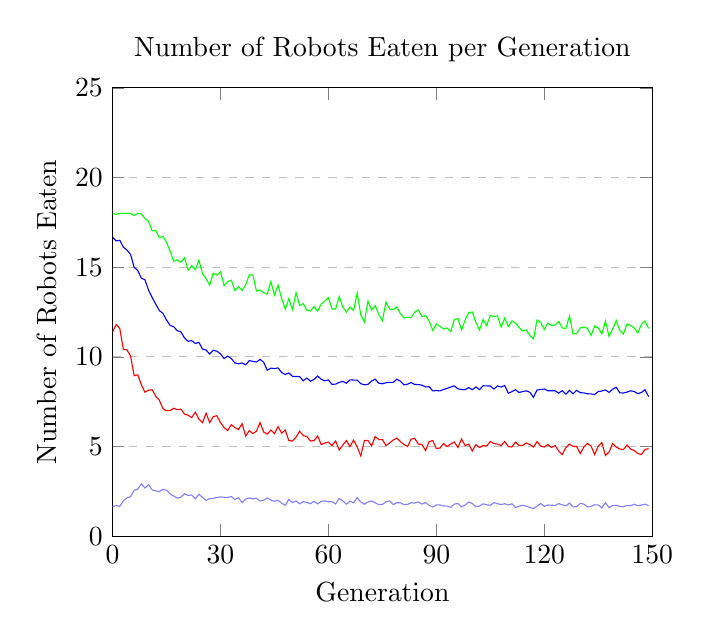
\begin{tikzpicture}
\begin{axis}[
	title={Number of Robots Eaten per Generation},
	xlabel={Generation},
	ylabel={Number of Robots Eaten},
	xmin=0, xmax=150,
	ymin=0, ymax=25,
	xtick={0.0,30.0,60.0,90.0,120.0,150.0},
	ytick={0.0,5.0,10.0,15.0,20.0,25.0},
	ymajorgrids=true,
	grid style=dashed,
]

\addplot[
	color=green,
	]
	coordinates {
	(0,18.0)(1,17.944444444444443)(2,18.0)(3,18.0)(4,18.0)(5,18.0)(6,17.88888888888889)(7,18.0)(8,17.97222222222222)(9,17.72222222222222)(10,17.555555555555557)(11,17.02777777777778)(12,17.055555555555557)(13,16.63888888888889)(14,16.72222222222222)(15,16.38888888888889)(16,15.88888888888889)(17,15.333333333333334)(18,15.416666666666666)(19,15.277777777777777)(20,15.527777777777775)(21,14.833333333333334)(22,15.083333333333334)(23,14.861111111111109)(24,15.388888888888891)(25,14.638888888888888)(26,14.361111111111109)(27,14.000000000000002)(28,14.666666666666666)(29,14.555555555555557)(30,14.75)(31,13.972222222222221)(32,14.194444444444445)(33,14.277777777777779)(34,13.694444444444446)(35,13.916666666666668)(36,13.694444444444446)(37,14.027777777777777)(38,14.583333333333334)(39,14.555555555555557)(40,13.666666666666668)(41,13.722222222222223)(42,13.583333333333336)(43,13.499999999999996)(44,14.194444444444445)(45,13.444444444444446)(46,14.0)(47,13.25)(48,12.666666666666668)(49,13.25)(50,12.638888888888891)(51,13.58333333333333)(52,12.861111111111112)(53,12.972222222222221)(54,12.611111111111107)(55,12.555555555555554)(56,12.805555555555555)(57,12.555555555555555)(58,12.944444444444445)(59,13.111111111111112)(60,13.305555555555557)(61,12.666666666666664)(62,12.666666666666668)(63,13.36111111111111)(64,12.777777777777777)(65,12.500000000000002)(66,12.777777777777779)(67,12.583333333333332)(68,13.555555555555555)(69,12.333333333333334)(70,11.944444444444441)(71,13.111111111111109)(72,12.611111111111109)(73,12.86111111111111)(74,12.361111111111112)(75,12.027777777777777)(76,13.055555555555555)(77,12.666666666666668)(78,12.63888888888889)(79,12.777777777777777)(80,12.416666666666668)(81,12.166666666666666)(82,12.22222222222222)(83,12.194444444444445)(84,12.5)(85,12.611111111111114)(86,12.250000000000002)(87,12.305555555555555)(88,12.0)(89,11.472222222222221)(90,11.833333333333332)(91,11.694444444444445)(92,11.555555555555557)(93,11.611111111111112)(94,11.416666666666668)(95,12.083333333333334)(96,12.13888888888889)(97,11.5)(98,12.055555555555554)(99,12.472222222222221)(100,12.5)(101,11.916666666666666)(102,11.500000000000002)(103,12.083333333333334)(104,11.750000000000002)(105,12.305555555555555)(106,12.249999999999998)(107,12.277777777777775)(108,11.666666666666668)(109,12.166666666666666)(110,11.694444444444443)(111,12.0)(112,11.88888888888889)(113,11.63888888888889)(114,11.444444444444446)(115,11.5)(116,11.194444444444446)(117,10.999999999999998)(118,12.055555555555555)(119,11.916666666666666)(120,11.527777777777779)(121,11.888888888888888)(122,11.750000000000004)(123,11.777777777777777)(124,11.972222222222221)(125,11.611111111111112)(126,11.583333333333334)(127,12.277777777777779)(128,11.27777777777778)(129,11.305555555555557)(130,11.611111111111112)(131,11.666666666666668)(132,11.583333333333334)(133,11.194444444444445)(134,11.722222222222225)(135,11.61111111111111)(136,11.277777777777779)(137,12.000000000000002)(138,11.138888888888888)(139,11.555555555555557)(140,12.027777777777779)(141,11.472222222222221)(142,11.277777777777777)(143,11.833333333333334)(144,11.75)(145,11.61111111111111)(146,11.333333333333334)(147,11.805555555555555)(148,12.0)(149,11.583333333333332)
	};
\addplot[
	color=blue,
	]
	coordinates {
	(0,16.666666666666668)(1,16.46527777777778)(2,16.50115740740741)(3,16.118055555555557)(4,15.954861111111112)(5,15.710648148148149)(6,14.997685185185187)(7,14.815972222222223)(8,14.390046296296298)(9,14.29861111111111)(10,13.722222222222223)(11,13.310185185185187)(12,12.940972222222221)(13,12.583333333333334)(14,12.422453703703706)(15,12.05787037037037)(16,11.753472222222223)(17,11.679398148148149)(18,11.457175925925927)(19,11.395833333333332)(20,11.049768518518517)(21,10.868055555555555)(22,10.902777777777777)(23,10.747685185185187)(24,10.807870370370372)(25,10.4375)(26,10.380787037037038)(27,10.153935185185185)(28,10.37037037037037)(29,10.3125)(30,10.166666666666668)(31,9.903935185185185)(32,10.042824074074074)(33,9.90625)(34,9.66087962962963)(35,9.61574074074074)(36,9.658564814814815)(37,9.555555555555554)(38,9.788194444444445)(39,9.750000000000002)(40,9.712962962962964)(41,9.86111111111111)(42,9.699074074074074)(43,9.254629629629628)(44,9.372685185185185)(45,9.346064814814815)(46,9.386574074074073)(47,9.12962962962963)(48,9.018518518518519)(49,9.105324074074074)(50,8.914351851851851)(51,8.912037037037038)(52,8.895833333333332)(53,8.667824074074073)(54,8.820601851851851)(55,8.640046296296296)(56,8.743055555555555)(57,8.934027777777779)(58,8.747685185185185)(59,8.66550925925926)(60,8.715277777777777)(61,8.465277777777777)(62,8.48263888888889)(63,8.57638888888889)(64,8.633101851851851)(65,8.528935185185185)(66,8.719907407407408)(67,8.706018518518519)(68,8.70486111111111)(69,8.508101851851851)(70,8.440972222222221)(71,8.467592592592593)(72,8.65162037037037)(73,8.75925925925926)(74,8.532407407407408)(75,8.498842592592592)(76,8.55787037037037)(77,8.57986111111111)(78,8.576388888888891)(79,8.753472222222221)(80,8.643518518518519)(81,8.435185185185185)(82,8.480324074074073)(83,8.568287037037038)(84,8.458333333333332)(85,8.45486111111111)(86,8.421296296296298)(87,8.322916666666666)(88,8.337962962962964)(89,8.101851851851851)(90,8.119212962962964)(91,8.10300925925926)(92,8.181712962962962)(93,8.24537037037037)(94,8.319444444444445)(95,8.381944444444445)(96,8.219907407407408)(97,8.174768518518517)(98,8.168981481481481)(99,8.28587962962963)(100,8.166666666666666)(101,8.322916666666668)(102,8.174768518518517)(103,8.388888888888888)(104,8.379629629629632)(105,8.373842592592593)(106,8.206018518518517)(107,8.376157407407408)(108,8.314814814814815)(109,8.406250000000002)(110,7.969907407407407)(111,8.062500000000002)(112,8.166666666666668)(113,8.008101851851851)(114,8.070601851851853)(115,8.104166666666666)(116,8.024305555555555)(117,7.74537037037037)(118,8.15162037037037)(119,8.179398148148147)(120,8.208333333333334)(121,8.11111111111111)(122,8.108796296296294)(123,8.109953703703702)(124,7.976851851851851)(125,8.113425925925927)(126,7.9131944444444455)(127,8.128472222222223)(128,7.939814814814813)(129,8.13425925925926)(130,8.002314814814815)(131,7.991898148148149)(132,7.943287037037038)(133,7.934027777777779)(134,7.900462962962964)(135,8.064814814814817)(136,8.097222222222221)(137,8.153935185185185)(138,8.018518518518519)(139,8.194444444444445)(140,8.30324074074074)(141,7.9907407407407405)(142,7.986111111111111)(143,8.035879629629628)(144,8.108796296296296)(145,8.06712962962963)(146,7.949074074074074)(147,8.012731481481483)(148,8.171296296296296)(149,7.780092592592593)
	};
\addplot[
	color=red,
	]
	coordinates {
	(0,11.38888888888889)(1,11.805555555555555)(2,11.583333333333334)(3,10.416666666666664)(4,10.38888888888889)(5,10.055555555555555)(6,8.944444444444445)(7,9.0)(8,8.444444444444445)(9,8.027777777777779)(10,8.13888888888889)(11,8.166666666666666)(12,7.8055555555555545)(13,7.583333333333334)(14,7.111111111111111)(15,7.0)(16,6.999999999999999)(17,7.138888888888889)(18,7.055555555555556)(19,7.083333333333333)(20,6.805555555555555)(21,6.75)(22,6.611111111111111)(23,6.916666666666667)(24,6.527777777777777)(25,6.333333333333332)(26,6.861111111111111)(27,6.333333333333333)(28,6.666666666666667)(29,6.722222222222222)(30,6.333333333333333)(31,6.055555555555555)(32,5.888888888888889)(33,6.222222222222222)(34,6.055555555555556)(35,5.944444444444444)(36,6.277777777777778)(37,5.583333333333334)(38,5.888888888888888)(39,5.722222222222222)(40,5.861111111111112)(41,6.333333333333334)(42,5.805555555555556)(43,5.6944444444444455)(44,5.916666666666666)(45,5.722222222222222)(46,6.111111111111111)(47,5.75)(48,5.916666666666667)(49,5.333333333333334)(50,5.305555555555556)(51,5.527777777777778)(52,5.861111111111112)(53,5.611111111111111)(54,5.555555555555556)(55,5.3055555555555545)(56,5.333333333333332)(57,5.583333333333334)(58,5.111111111111111)(59,5.194444444444445)(60,5.25)(61,5.055555555555556)(62,5.305555555555555)(63,4.805555555555555)(64,5.083333333333334)(65,5.333333333333333)(66,5.000000000000001)(67,5.361111111111111)(68,4.972222222222222)(69,4.472222222222222)(70,5.333333333333334)(71,5.333333333333334)(72,5.027777777777778)(73,5.5555555555555545)(74,5.388888888888888)(75,5.388888888888888)(76,5.055555555555555)(77,5.194444444444445)(78,5.361111111111111)(79,5.472222222222221)(80,5.277777777777777)(81,5.111111111111112)(82,5.000000000000001)(83,5.416666666666667)(84,5.444444444444444)(85,5.138888888888889)(86,5.111111111111111)(87,4.777777777777778)(88,5.277777777777779)(89,5.333333333333333)(90,4.888888888888889)(91,4.916666666666667)(92,5.166666666666666)(93,5.0)(94,5.138888888888889)(95,5.25)(96,4.944444444444444)(97,5.416666666666667)(98,5.055555555555556)(99,5.138888888888888)(100,4.75)(101,5.111111111111112)(102,4.944444444444445)(103,5.055555555555556)(104,5.027777777777778)(105,5.277777777777779)(106,5.166666666666667)(107,5.138888888888889)(108,5.055555555555555)(109,5.277777777777778)(110,5.0)(111,4.972222222222221)(112,5.250000000000001)(113,5.055555555555556)(114,5.055555555555555)(115,5.194444444444445)(116,5.111111111111111)(117,4.972222222222221)(118,5.277777777777778)(119,5.027777777777777)(120,4.972222222222221)(121,5.111111111111112)(122,4.9444444444444455)(123,5.055555555555555)(124,4.75)(125,4.555555555555555)(126,4.944444444444445)(127,5.138888888888888)(128,5.0)(129,5.0)(130,4.611111111111111)(131,4.972222222222222)(132,5.166666666666666)(133,5.027777777777777)(134,4.555555555555555)(135,5.027777777777778)(136,5.222222222222223)(137,4.5)(138,4.694444444444444)(139,5.166666666666667)(140,4.972222222222222)(141,4.8611111111111125)(142,4.833333333333333)(143,5.083333333333333)(144,4.861111111111111)(145,4.777777777777778)(146,4.611111111111112)(147,4.555555555555555)(148,4.833333333333334)(149,4.888888888888889)
	};
\addplot[
	color=blue!50,
	]
	coordinates {
	(0,1.6393905375946907)(1,1.718786720766471)(2,1.656673884659449)(3,1.9803525230540049)(4,2.136449308171987)(5,2.2025436011445607)(6,2.557892021483334)(7,2.623712519083635)(8,2.9258766819151916)(9,2.688614374719867)(10,2.873693759083144)(11,2.580373241892872)(12,2.5268823613670506)(13,2.490343930620755)(14,2.6075349995175774)(15,2.568634117627958)(16,2.3524285561926837)(17,2.2396329782326108)(18,2.1255813065287192)(19,2.174626148972705)(20,2.3670764648064146)(21,2.273284883640197)(22,2.2966692965588944)(23,2.0816011585373664)(24,2.3413565602147486)(25,2.160942908982197)(26,2.001554282489532)(27,2.0895766631747823)(28,2.1062630413495085)(29,2.1605933877321255)(30,2.1918589775534896)(31,2.1700430796228156)(32,2.1571193895017857)(33,2.2174692439717916)(34,2.0415449546073665)(35,2.1480452955585925)(36,1.8681306261253883)(37,2.072060737374949)(38,2.132155154817689)(39,2.083356468550907)(40,2.1072490219897713)(41,1.9657039611472187)(42,2.0034455129921716)(43,2.132539084446683)(44,2.0160497854502233)(45,1.946782249236461)(46,2.0070020991189814)(47,1.8431583730624281)(48,1.717016868171965)(49,2.053107480661297)(50,1.8775983869213964)(51,1.9619059122766744)(52,1.8099812108415423)(53,1.923860657006745)(54,1.8856980349075723)(55,1.809685760814311)(56,1.9430254329197474)(57,1.8033021850938917)(58,1.9413180268461832)(59,1.9668431153007377)(60,1.9200692186989787)(61,1.9234180927149418)(62,1.7982008595214143)(63,2.1017066875815096)(64,1.969464379678767)(65,1.78643978788816)(66,1.949855716830367)(67,1.8586360430833029)(68,2.1486230263768427)(69,1.9128909312103897)(70,1.7781863247072922)(71,1.9139112696136986)(72,1.9585410335521163)(73,1.8675119359567796)(74,1.7606762514763266)(75,1.774346886130343)(76,1.9195682311470825)(77,1.9702566244788065)(78,1.7644271919362013)(79,1.863874233890743)(80,1.8622181555199098)(81,1.7591925848225833)(82,1.774389068585374)(83,1.8656248425358715)(84,1.8481230628626013)(85,1.9103997760120077)(86,1.7895489675486178)(87,1.8794083951307283)(88,1.7202162107318264)(89,1.62294209979586)(90,1.7458159787349232)(91,1.7419635566411273)(92,1.6854834631782485)(93,1.6762282088456208)(94,1.6145003145674255)(95,1.791914204011709)(96,1.8237178469157043)(97,1.6425078881159383)(98,1.7427593529452095)(99,1.9099663189417169)(100,1.819322387970391)(101,1.639794853676872)(102,1.6834221557391673)(103,1.8070030347425865)(104,1.7486264547211685)(105,1.7251967292107766)(106,1.872503658711875)(107,1.8127572918236097)(108,1.7628484547763585)(109,1.8117324931885372)(110,1.739514402732164)(111,1.806785044537857)(112,1.597158767063146)(113,1.677694282419649)(114,1.7235194638511635)(115,1.6742484894200054)(116,1.6017065342960388)(117,1.5412728300291194)(118,1.677602672590296)(119,1.821068080721953)(120,1.6685212018139042)(121,1.742090475693624)(122,1.7287244152431844)(123,1.7112233457745545)(124,1.8177440977436756)(125,1.7497541817353817)(126,1.6924836510678867)(127,1.8426060979177945)(128,1.6338730268967412)(129,1.6489171310692794)(130,1.8300124398482205)(131,1.7904164470619741)(132,1.6359667563498208)(133,1.6592614385487048)(134,1.7531463561789087)(135,1.740668194215493)(136,1.581590508073917)(137,1.868994311440664)(138,1.594857649287079)(139,1.7052053270879672)(140,1.7238850274795985)(141,1.6601765537719675)(142,1.6440016524344154)(143,1.7171834421426502)(144,1.6979315648861402)(145,1.7792095328191238)(146,1.698422167169895)(147,1.7359269300525855)(148,1.7831439550578045)(149,1.703679353116592)
	};
\end{axis}
\end{tikzpicture}
}
		\caption{Some sample caption}
		\label{fig:easy-robots-eaten}
	\end{subfigure}%
}
\\
\\
\\
	\makebox[\linewidth][c]{%
	\begin{subfigure}[b]{0.7\textwidth}
		\centering
		\resizebox{0.9\linewidth}{!}{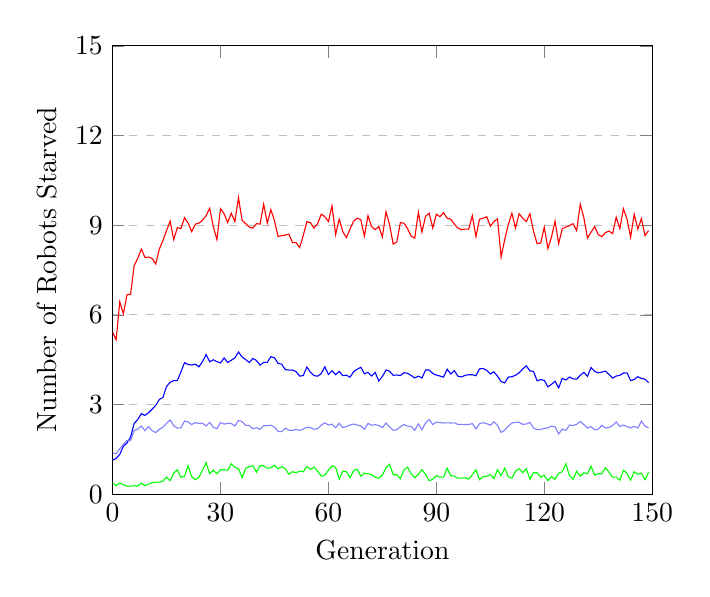
\begin{tikzpicture}
\begin{axis}[
	xlabel={Generation},
	ylabel={Number of Robots Starved},
	xmin=0, xmax=150,
	ymin=0, ymax=15,
	xtick={0.0,30.0,60.0,90.0,120.0,150.0},
	ytick={0.0,3.0,6.0,9.0,12.0,15.0},
	ymajorgrids=true,
	grid style=dashed,
]

\addplot[
	color=red,
	]
	coordinates {
	(0,5.416666666666667)(1,5.166666666666666)(2,6.4333333333333345)(3,6.033333333333332)(4,6.666666666666666)(5,6.6833333333333345)(6,7.649999999999999)(7,7.883333333333334)(8,8.200000000000001)(9,7.916666666666666)(10,7.933333333333334)(11,7.883333333333335)(12,7.7)(13,8.200000000000001)(14,8.483333333333333)(15,8.816666666666666)(16,9.133333333333333)(17,8.516666666666666)(18,8.916666666666666)(19,8.883333333333335)(20,9.25)(21,9.066666666666665)(22,8.783333333333335)(23,9.033333333333331)(24,9.066666666666665)(25,9.166666666666668)(26,9.316666666666665)(27,9.566666666666666)(28,8.95)(29,8.516666666666667)(30,9.55)(31,9.383333333333333)(32,9.083333333333332)(33,9.4)(34,9.116666666666667)(35,9.916666666666668)(36,9.166666666666668)(37,9.049999999999999)(38,8.933333333333332)(39,8.9)(40,9.05)(41,9.033333333333333)(42,9.700000000000001)(43,9.066666666666666)(44,9.516666666666667)(45,9.149999999999999)(46,8.616666666666665)(47,8.65)(48,8.666666666666668)(49,8.700000000000001)(50,8.416666666666668)(51,8.416666666666666)(52,8.25)(53,8.649999999999999)(54,9.116666666666665)(55,9.083333333333334)(56,8.899999999999999)(57,9.05)(58,9.366666666666665)(59,9.283333333333331)(60,9.116666666666665)(61,9.65)(62,8.683333333333334)(63,9.200000000000001)(64,8.783333333333335)(65,8.583333333333336)(66,8.866666666666665)(67,9.133333333333333)(68,9.233333333333333)(69,9.183333333333332)(70,8.633333333333335)(71,9.316666666666666)(72,8.950000000000001)(73,8.85)(74,8.950000000000001)(75,8.6)(76,9.45)(77,9.016666666666666)(78,8.366666666666667)(79,8.433333333333332)(80,9.083333333333332)(81,9.066666666666666)(82,8.883333333333333)(83,8.633333333333333)(84,8.566666666666668)(85,9.433333333333332)(86,8.766666666666667)(87,9.299999999999999)(88,9.399999999999999)(89,8.899999999999999)(90,9.366666666666665)(91,9.283333333333333)(92,9.416666666666668)(93,9.233333333333333)(94,9.2)(95,9.033333333333331)(96,8.899999999999999)(97,8.85)(98,8.866666666666667)(99,8.866666666666667)(100,9.316666666666666)(101,8.616666666666665)(102,9.199999999999998)(103,9.233333333333334)(104,9.283333333333331)(105,8.966666666666667)(106,9.116666666666665)(107,9.216666666666667)(108,7.933333333333332)(109,8.516666666666667)(110,9.016666666666666)(111,9.400000000000002)(112,8.900000000000002)(113,9.383333333333333)(114,9.233333333333333)(115,9.116666666666667)(116,9.383333333333335)(117,8.8)(118,8.383333333333333)(119,8.4)(120,8.933333333333332)(121,8.216666666666667)(122,8.600000000000001)(123,9.133333333333335)(124,8.383333333333333)(125,8.883333333333333)(126,8.933333333333334)(127,8.983333333333334)(128,9.049999999999999)(129,8.816666666666668)(130,9.7)(131,9.25)(132,8.566666666666666)(133,8.766666666666667)(134,8.950000000000001)(135,8.683333333333334)(136,8.616666666666665)(137,8.749999999999998)(138,8.799999999999999)(139,8.716666666666667)(140,9.266666666666667)(141,8.883333333333333)(142,9.549999999999999)(143,9.2)(144,8.6)(145,9.366666666666667)(146,8.866666666666665)(147,9.216666666666667)(148,8.65)(149,8.816666666666668)
	};
\addplot[
	color=blue,
	]
	coordinates {
	(0,1.1395833333333334)(1,1.190972222222222)(2,1.3319444444444444)(3,1.6055555555555554)(4,1.7069444444444448)(5,1.904166666666667)(6,2.3618055555555557)(7,2.495138888888889)(8,2.6944444444444446)(9,2.6347222222222224)(10,2.722916666666667)(11,2.8444444444444446)(12,2.9673611111111113)(13,3.1680555555555556)(14,3.234027777777778)(15,3.599999999999999)(16,3.74375)(17,3.7972222222222216)(18,3.797916666666667)(19,4.088194444444444)(20,4.4006944444444445)(21,4.335416666666667)(22,4.319444444444444)(23,4.347916666666666)(24,4.258333333333334)(25,4.434027777777777)(26,4.667361111111111)(27,4.428472222222222)(28,4.495138888888889)(29,4.434722222222222)(30,4.388888888888888)(31,4.558333333333334)(32,4.405555555555556)(33,4.479166666666666)(34,4.558333333333333)(35,4.754861111111112)(36,4.5875)(37,4.502083333333333)(38,4.40625)(39,4.5375)(40,4.470833333333333)(41,4.317361111111111)(42,4.405555555555556)(43,4.406944444444446)(44,4.598611111111111)(45,4.559027777777778)(46,4.375)(47,4.345833333333333)(48,4.16875)(49,4.149305555555555)(50,4.152083333333334)(51,4.1006944444444455)(52,3.948611111111111)(53,3.966666666666666)(54,4.250000000000001)(55,4.08125)(56,3.963888888888889)(57,3.9465277777777774)(58,4.030555555555556)(59,4.259027777777777)(60,4.004166666666667)(61,4.124305555555555)(62,3.9972222222222236)(63,4.106944444444444)(64,3.963888888888889)(65,3.9805555555555556)(66,3.9111111111111105)(67,4.095138888888889)(68,4.178472222222222)(69,4.24375)(70,4.027777777777778)(71,4.072916666666667)(72,3.9520833333333334)(73,4.070833333333334)(74,3.7840277777777778)(75,3.938888888888889)(76,4.1506944444444445)(77,4.110416666666667)(78,3.9763888888888883)(79,3.9854166666666666)(80,3.968055555555555)(81,4.061805555555556)(82,4.043055555555556)(83,3.969444444444444)(84,3.888888888888889)(85,3.947222222222223)(86,3.885416666666666)(87,4.151388888888889)(88,4.154166666666668)(89,4.035416666666667)(90,3.983333333333334)(91,3.951388888888888)(92,3.9138888888888896)(93,4.180555555555555)(94,4.020138888888889)(95,4.13125)(96,3.9451388888888888)(97,3.920833333333334)(98,3.9770833333333324)(99,3.9944444444444454)(100,3.995138888888888)(101,3.960416666666667)(102,4.190972222222222)(103,4.205555555555556)(104,4.142361111111112)(105,4.018055555555556)(106,4.093055555555556)(107,3.9458333333333337)(108,3.769444444444445)(109,3.720138888888888)(110,3.916666666666666)(111,3.9277777777777776)(112,3.9791666666666665)(113,4.055555555555555)(114,4.188194444444445)(115,4.293055555555556)(116,4.122222222222223)(117,4.1090277777777775)(118,3.7916666666666665)(119,3.830555555555556)(120,3.8069444444444445)(121,3.590972222222222)(122,3.6729166666666666)(123,3.7784722222222227)(124,3.5548611111111112)(125,3.8756944444444446)(126,3.817361111111111)(127,3.9194444444444443)(128,3.8583333333333334)(129,3.8458333333333337)(130,3.9750000000000005)(131,4.074305555555556)(132,3.9402777777777773)(133,4.235416666666666)(134,4.106249999999999)(135,4.060416666666667)(136,4.083333333333333)(137,4.113888888888889)(138,4.0055555555555555)(139,3.8833333333333333)(140,3.952083333333334)(141,3.9743055555555555)(142,4.052777777777778)(143,4.05625)(144,3.7986111111111116)(145,3.8354166666666667)(146,3.9291666666666667)(147,3.8715277777777772)(148,3.845833333333334)(149,3.7236111111111105)
	};
\addplot[
	color=green,
	]
	coordinates {
	(0,0.3833333333333333)(1,0.2833333333333333)(2,0.36666666666666664)(3,0.31666666666666665)(4,0.26666666666666666)(5,0.26666666666666666)(6,0.2833333333333333)(7,0.26666666666666666)(8,0.36666666666666664)(9,0.2833333333333333)(10,0.3333333333333333)(11,0.3833333333333333)(12,0.39999999999999997)(13,0.39999999999999997)(14,0.4333333333333333)(15,0.5666666666666667)(16,0.44999999999999996)(17,0.7000000000000001)(18,0.8166666666666667)(19,0.5666666666666668)(20,0.6000000000000001)(21,0.9500000000000002)(22,0.5833333333333334)(23,0.48333333333333334)(24,0.5666666666666667)(25,0.7999999999999999)(26,1.0500000000000003)(27,0.6833333333333332)(28,0.8)(29,0.6833333333333333)(30,0.8166666666666667)(31,0.8166666666666667)(32,0.8)(33,1.0166666666666668)(34,0.9)(35,0.85)(36,0.5500000000000002)(37,0.8666666666666668)(38,0.9166666666666669)(39,0.9500000000000003)(40,0.7333333333333335)(41,0.9500000000000002)(42,0.95)(43,0.8666666666666668)(44,0.8833333333333334)(45,0.9666666666666667)(46,0.85)(47,0.9166666666666667)(48,0.85)(49,0.6666666666666667)(50,0.7500000000000001)(51,0.7166666666666667)(52,0.7666666666666666)(53,0.75)(54,0.9166666666666669)(55,0.8333333333333335)(56,0.9)(57,0.7666666666666666)(58,0.6000000000000001)(59,0.6333333333333335)(60,0.8)(61,0.9500000000000001)(62,0.9000000000000001)(63,0.49999999999999994)(64,0.7666666666666666)(65,0.7500000000000001)(66,0.55)(67,0.7833333333333334)(68,0.8333333333333335)(69,0.6)(70,0.7000000000000001)(71,0.6833333333333335)(72,0.65)(73,0.5666666666666668)(74,0.5333333333333333)(75,0.6333333333333333)(76,0.8833333333333333)(77,1.0000000000000002)(78,0.65)(79,0.6499999999999999)(80,0.5166666666666666)(81,0.8166666666666668)(82,0.9)(83,0.6833333333333335)(84,0.5500000000000002)(85,0.6666666666666667)(86,0.8166666666666667)(87,0.6666666666666667)(88,0.44999999999999996)(89,0.49999999999999994)(90,0.6166666666666668)(91,0.5666666666666667)(92,0.5666666666666667)(93,0.8666666666666668)(94,0.6166666666666667)(95,0.6000000000000001)(96,0.5333333333333333)(97,0.5333333333333334)(98,0.55)(99,0.5)(100,0.65)(101,0.8166666666666667)(102,0.4833333333333333)(103,0.5833333333333334)(104,0.6)(105,0.6499999999999999)(106,0.5166666666666666)(107,0.8166666666666668)(108,0.6166666666666668)(109,0.8666666666666668)(110,0.5833333333333333)(111,0.5333333333333334)(112,0.7666666666666667)(113,0.85)(114,0.7166666666666667)(115,0.8500000000000001)(116,0.49999999999999994)(117,0.7166666666666667)(118,0.7166666666666667)(119,0.5666666666666667)(120,0.6333333333333333)(121,0.44999999999999996)(122,0.5833333333333334)(123,0.49999999999999994)(124,0.7)(125,0.7500000000000003)(126,1.0166666666666668)(127,0.6166666666666667)(128,0.5)(129,0.7666666666666666)(130,0.6)(131,0.7166666666666667)(132,0.6833333333333335)(133,0.9333333333333335)(134,0.6333333333333333)(135,0.6833333333333333)(136,0.6833333333333335)(137,0.8833333333333335)(138,0.7333333333333334)(139,0.5666666666666667)(140,0.5666666666666667)(141,0.4666666666666666)(142,0.8)(143,0.7)(144,0.4666666666666666)(145,0.75)(146,0.6666666666666667)(147,0.7)(148,0.48333333333333334)(149,0.7333333333333334)
	};
\addplot[
	color=blue!50,
	]
	coordinates {
	(0,1.3740761608251102)(1,1.3500170192659637)(2,1.5210624858350448)(3,1.6672246833461069)(4,1.794468112824373)(5,1.7945906267009162)(6,2.124776740772433)(7,2.1756514515631644)(8,2.2800344886364683)(9,2.1224477771120203)(10,2.2588658274861695)(11,2.1239877374180303)(12,2.058688468923767)(13,2.166429849847634)(14,2.2363112748055634)(15,2.3707864305068305)(16,2.479569570625487)(17,2.285188115411621)(18,2.210727043233327)(19,2.220527036615759)(20,2.4452238754240914)(21,2.4153216344914017)(22,2.328430219879035)(23,2.3939957313150164)(24,2.364070930714652)(25,2.377337806304615)(26,2.281760412605469)(27,2.401463844841529)(28,2.237347025148171)(29,2.1876366742497497)(30,2.3986375104577555)(31,2.343694922171343)(32,2.368037432798033)(33,2.364497211644153)(34,2.2795460538208734)(35,2.464296486952522)(36,2.425059056494363)(37,2.2977110730841903)(38,2.2992266097221923)(39,2.1847734780986476)(40,2.2204336170333017)(41,2.1691130185917378)(42,2.2858964488944844)(43,2.2928790642813475)(44,2.3046036036274407)(45,2.24030437366637)(46,2.099518296409575)(47,2.0894376572733373)(48,2.2098468284761896)(49,2.139116425637767)(50,2.1312849004320373)(51,2.1631871456725733)(52,2.1319719936109727)(53,2.174245228673195)(54,2.2433293091778985)(55,2.2251703907573903)(56,2.1705024617759454)(57,2.190247072646373)(58,2.3072226248201915)(59,2.3896031291996636)(60,2.309906635222237)(61,2.3429758014026523)(62,2.219559817597767)(63,2.3737124557764937)(64,2.22759514638622)(65,2.260500385077578)(66,2.312461866241447)(67,2.345717328177497)(68,2.310669264036696)(69,2.283908470256852)(70,2.1691688953692982)(71,2.3647197747731266)(72,2.302972074914847)(73,2.324566145573782)(74,2.295016335190698)(75,2.2211352065569856)(76,2.3792206445779884)(77,2.2440969259544365)(78,2.1374645116419977)(79,2.1494983121719327)(80,2.2567811538547193)(81,2.3260764469570363)(82,2.276341473251344)(83,2.260761891387623)(84,2.136249405054538)(85,2.3505091331167436)(86,2.1547216308607866)(87,2.3809422529746125)(88,2.494304886405157)(89,2.3294481951868597)(90,2.406811638368797)(91,2.3931068956635873)(92,2.3803531540001703)(93,2.3861511613506443)(94,2.3795484979720185)(95,2.386145566615623)(96,2.3323247802125846)(97,2.3328219381858806)(98,2.3290668351297596)(99,2.328300010746401)(100,2.361170671144893)(101,2.181798180547283)(102,2.3576361725173243)(103,2.3877388553346113)(104,2.35709874897104)(105,2.30698325720816)(106,2.4195652842789555)(107,2.297705522137604)(108,2.0627779734129756)(109,2.1363477710620966)(110,2.2741038100311624)(111,2.377680883307688)(112,2.399262988165911)(113,2.4044217716535607)(114,2.3370921881694477)(115,2.3435314042233415)(116,2.4010708422648537)(117,2.2080787144758203)(118,2.1552634628436205)(119,2.1667399917116663)(120,2.197783154313116)(121,2.216843046305531)(122,2.275357054661697)(123,2.251493342409839)(124,2.012387378850751)(125,2.177811574025096)(126,2.1299459797978475)(127,2.311254399040608)(128,2.2962386835181023)(129,2.3341679490570804)(130,2.4337314621758463)(131,2.3267780097490602)(132,2.2127271658923635)(133,2.2600752664332417)(134,2.150562640222129)(135,2.1750108614738113)(136,2.300877912512625)(137,2.214634182650521)(138,2.2271954296463146)(139,2.295120210758526)(140,2.4170159689577484)(141,2.2624344989133482)(142,2.3141827058683297)(143,2.2571344860981486)(144,2.218798854025148)(145,2.2701279650694612)(146,2.2118317162541836)(147,2.4406310721652114)(148,2.27458069540652)(149,2.2220890960067035)
	};
\end{axis}
\end{tikzpicture}
}
		\caption{Some sample caption}
		\label{fig:easy-robots-starved}
	\end{subfigure}%
	\begin{subfigure}[b]{0.7\textwidth}
		\centering
		\resizebox{0.9\linewidth}{!}{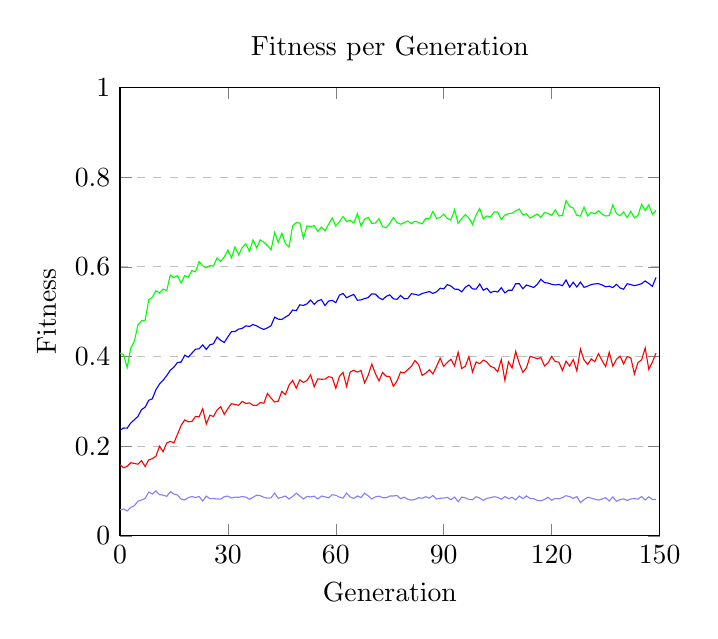
\begin{tikzpicture}
\begin{axis}[
	title={Fitness per Generation},
	xlabel={Generation},
	ylabel={Fitness},
	xmin=0, xmax=150,
	ymin=0, ymax=1,
	xtick={0.0,30.0,60.0,90.0,120.0,150.0},
	ytick={0.0,0.2,0.4,0.6000000000000001,0.8,1.0},
	ymajorgrids=true,
	grid style=dashed,
]

\addplot[
	color=green,
	]
	coordinates {
	(0,0.407433024691358)(1,0.40455246913580245)(2,0.375249537037037)(3,0.41873225308641987)(4,0.43406728395061733)(5,0.47047870370370376)(6,0.48000061728395077)(7,0.48074444444444436)(8,0.5266174382716049)(9,0.5326043209876542)(10,0.546644598765432)(11,0.5416791666666666)(12,0.550737037037037)(13,0.5472788580246913)(14,0.5818168209876543)(15,0.5762845679012346)(16,0.5803973765432099)(17,0.5637412037037037)(18,0.5807561728395062)(19,0.5770462962962962)(20,0.5918933641975308)(21,0.5890060185185186)(22,0.611758024691358)(23,0.6023779320987654)(24,0.597986574074074)(25,0.6028320987654322)(26,0.6018344135802469)(27,0.6198837962962963)(28,0.6122495370370372)(29,0.6220623456790124)(30,0.6373035493827159)(31,0.6203790123456789)(32,0.6443311728395062)(33,0.6266847222222223)(34,0.6429742283950617)(35,0.6516114197530866)(36,0.6346967592592594)(37,0.6601297839506174)(38,0.6424608024691357)(39,0.6603320987654321)(40,0.6550021604938272)(41,0.6473228395061729)(42,0.6378552469135802)(43,0.6765921296296297)(44,0.6545077160493827)(45,0.67522762345679)(46,0.6522231481481482)(47,0.6441180555555557)(48,0.6918532407407407)(49,0.6986695987654321)(50,0.6978850308641976)(51,0.6640128086419752)(52,0.6916970679012346)(53,0.6898421296296298)(54,0.6921731481481481)(55,0.6790364197530865)(56,0.6888367283950617)(57,0.6804623456790124)(58,0.6950320987654318)(59,0.7090398148148146)(60,0.6910038580246913)(61,0.7005773148148147)(62,0.7123285493827161)(63,0.701445987654321)(64,0.7039131172839507)(65,0.6975145061728395)(66,0.7190006172839506)(67,0.6912452160493827)(68,0.7063524691358025)(69,0.7106902777777777)(70,0.696969598765432)(71,0.6977742283950615)(72,0.7074362654320988)(73,0.6898623456790122)(74,0.6872458333333334)(75,0.6969765432098767)(76,0.7099206790123456)(77,0.699322685185185)(78,0.6952020061728394)(79,0.6986459876543211)(80,0.7024952160493828)(81,0.6961916666666669)(82,0.7019111111111112)(83,0.6990598765432098)(84,0.695925925925926)(85,0.7083817901234568)(86,0.7070557098765433)(87,0.7236819444444443)(88,0.7083805555555556)(89,0.7099149691358025)(90,0.7174049382716048)(91,0.7082470679012347)(92,0.7043149691358025)(93,0.7279672839506172)(94,0.6972297839506173)(95,0.7076268518518519)(96,0.7167833333333333)(97,0.7092716049382716)(98,0.6942013888888888)(99,0.7159430555555555)(100,0.7302199074074074)(101,0.7070033950617285)(102,0.7135929012345678)(103,0.7119015432098765)(104,0.7224578703703707)(105,0.7223239197530865)(106,0.7057788580246914)(107,0.7157495370370369)(108,0.7186895061728394)(109,0.7197694444444445)(110,0.7249671296296297)(111,0.7290618827160494)(112,0.7162617283950617)(113,0.7185904320987652)(114,0.7088546296296298)(115,0.7133479938271603)(116,0.71792237654321)(117,0.7102621913580247)(118,0.7212990740740741)(119,0.7193080246913581)(120,0.7151873456790123)(121,0.7271918209876542)(122,0.7135947530864198)(123,0.7149155864197531)(124,0.748066975308642)(125,0.73450987654321)(126,0.7312785493827161)(127,0.7150501543209877)(128,0.7132081790123458)(129,0.7334890432098767)(130,0.7137737654320988)(131,0.7214353395061728)(132,0.7183952160493826)(133,0.7253006172839508)(134,0.7177473765432097)(135,0.7134174382716051)(136,0.7144007716049384)(137,0.7385118827160495)(138,0.7191226851851853)(139,0.7142382716049382)(140,0.7225233024691359)(141,0.7100907407407406)(142,0.7240393518518519)(143,0.7093845679012346)(144,0.7148962962962964)(145,0.7397091049382715)(146,0.7257822530864197)(147,0.738746450617284)(148,0.7170873456790123)(149,0.7262729938271605)
	};
\addplot[
	color=blue,
	]
	coordinates {
	(0,0.23568551311728395)(1,0.24068541666666662)(2,0.24022112911522633)(3,0.25169717721193413)(4,0.2590899241255144)(5,0.2664853266460906)(6,0.28171860210905353)(7,0.2870059606481481)(8,0.3024511638374485)(9,0.30586267361111114)(10,0.3260418595679012)(11,0.338852070473251)(12,0.3473097029320988)(13,0.3574480195473251)(14,0.369612879372428)(15,0.3764822852366255)(16,0.38693112139917696)(17,0.38745133744855964)(18,0.40305448173868313)(19,0.39877369470164614)(20,0.40770316358024694)(21,0.41631231352880665)(22,0.417209921553498)(23,0.42592258873456784)(24,0.41594365997942395)(25,0.4262058513374486)(26,0.4285938078703704)(27,0.4435030671296296)(28,0.43614852752057603)(29,0.43139828960905346)(30,0.44385616640946496)(31,0.4555685635288066)(32,0.4559813914609053)(33,0.46119753086419757)(34,0.4630295910493827)(35,0.46848685699588477)(36,0.4671781121399177)(37,0.47134870113168725)(38,0.468452912808642)(39,0.4638823173868312)(40,0.4604523083847737)(41,0.46414776234567895)(42,0.46880528549382716)(43,0.48797928240740746)(44,0.4834216949588477)(45,0.48267862654320975)(46,0.48814235468107003)(47,0.4928079539609053)(48,0.5038436342592593)(49,0.5023217271090534)(50,0.5154713927469136)(51,0.5140101594650206)(52,0.5177034850823046)(53,0.5259832626028808)(54,0.5164022505144032)(55,0.5241722543724279)(56,0.5268482574588478)(57,0.5139078125000001)(58,0.5237850180041153)(59,0.5252607960390946)(60,0.5201704475308643)(61,0.5369881301440329)(62,0.5407399627057614)(63,0.5311644547325103)(64,0.5352260480967079)(65,0.5385806520061728)(66,0.5256074974279835)(67,0.5264563593106996)(68,0.5292461162551441)(69,0.5315578639403292)(70,0.5397327803497942)(71,0.5393159079218106)(72,0.5311407664609054)(73,0.5270274562757201)(74,0.5341304333847736)(75,0.537654140946502)(76,0.5289976466049382)(77,0.527455028292181)(78,0.5364096000514403)(79,0.5288648469650206)(80,0.5294152263374485)(81,0.5400965342078189)(82,0.5389623906893004)(83,0.5367551826131688)(84,0.5407509773662552)(85,0.5428390753600824)(86,0.5450959683641975)(87,0.54066875)(88,0.5444795717592592)(89,0.5525789030349794)(90,0.5508464441872428)(91,0.560527700617284)(92,0.5573773019547326)(93,0.5503285686728394)(94,0.5500769483024691)(95,0.5443369277263375)(96,0.5545731738683127)(97,0.5596265110596708)(98,0.5508877379115227)(99,0.5503951324588477)(100,0.5618264081790124)(101,0.5478969585905349)(102,0.5523157793209877)(103,0.5425106867283951)(104,0.5456846900720165)(105,0.543947633744856)(106,0.5536538966049382)(107,0.5419271219135802)(108,0.5479063657407407)(109,0.5477672260802469)(110,0.5625017554012345)(111,0.5624469071502058)(112,0.551313007973251)(113,0.5595609117798354)(114,0.5569121849279837)(115,0.5540847350823045)(116,0.5610753986625515)(117,0.572394045781893)(118,0.5649596129115226)(119,0.5639924382716048)(120,0.5611585390946502)(121,0.5596785236625514)(122,0.5608497620884774)(123,0.5581145640432099)(124,0.5709340534979425)(125,0.5549676826131686)(126,0.565735558127572)(127,0.5551598251028808)(128,0.5659945344650205)(129,0.5544160365226337)(130,0.5571219585905349)(131,0.5605994277263375)(132,0.5621280221193415)(133,0.5626246592078189)(134,0.5596513052983539)(135,0.555631880144033)(136,0.5569620177469135)(137,0.5538821180555557)(138,0.5610741190843622)(139,0.5530615162037038)(140,0.5501980259773662)(141,0.5625325360082304)(142,0.5604201903292181)(143,0.5582116576646091)(144,0.56005295781893)(145,0.5625418724279836)(146,0.568676517489712)(147,0.5630099408436213)(148,0.5567143840020575)(149,0.5763791538065843)
	};
\addplot[
	color=red,
	]
	coordinates {
	(0,0.15883472222222217)(1,0.15176620370370367)(2,0.15516774691358023)(3,0.16314398148148151)(4,0.16171574074074072)(5,0.1599047839506173)(6,0.167703549382716)(7,0.15460324074074072)(8,0.16965000000000008)(9,0.17227453703703707)(10,0.177687962962963)(11,0.20008703703703706)(12,0.1878003086419753)(13,0.20714043209876548)(14,0.21085910493827156)(15,0.2075063271604939)(16,0.2266248456790123)(17,0.2463229938271605)(18,0.2588023148148148)(19,0.25445648148148137)(20,0.2553297839506173)(21,0.2663185185185184)(22,0.26556466049382715)(23,0.28364907407407414)(24,0.24956651234567898)(25,0.26917608024691353)(26,0.266428086419753)(27,0.28083302469135807)(28,0.28820246913580233)(29,0.27107098765432097)(30,0.2839445987654321)(31,0.29507330246913577)(32,0.2930942901234568)(33,0.29139274691358025)(34,0.29994027777777776)(35,0.2953341049382716)(36,0.2966895061728395)(37,0.2912694444444444)(38,0.29084413580246915)(39,0.2974516975308642)(40,0.2958439814814814)(41,0.3177274691358025)(42,0.3072799382716051)(43,0.29868595679012344)(44,0.3005936728395062)(45,0.32242330246913586)(46,0.31510216049382717)(47,0.3362362654320988)(48,0.3466668209876543)(49,0.3295989197530865)(50,0.34805848765432096)(51,0.3424456790123457)(52,0.3466425925925927)(53,0.3592333333333333)(54,0.3325387345679012)(55,0.350087962962963)(56,0.3494266975308642)(57,0.3496253086419754)(58,0.35512654320987663)(59,0.3532475308641975)(60,0.3291945987654321)(61,0.3556766975308642)(62,0.3647975308641975)(63,0.333413425925926)(64,0.3656543209876543)(65,0.36919722222222223)(66,0.36540277777777774)(67,0.36901836419753076)(68,0.3412558641975309)(69,0.358175)(70,0.38318410493827154)(71,0.36207978395061735)(72,0.3456663580246913)(73,0.36432052469135806)(74,0.3562577160493827)(75,0.3551270061728395)(76,0.3336668209876544)(77,0.3450722222222221)(78,0.3654473765432099)(79,0.3635175925925926)(80,0.37078194444444446)(81,0.37806450617283943)(82,0.3910618827160493)(83,0.3824270061728395)(84,0.3579887345679014)(85,0.36289537037037034)(86,0.37047361111111116)(87,0.3612682098765431)(88,0.3780024691358025)(89,0.3961788580246913)(90,0.3779543209876544)(91,0.3867915123456791)(92,0.39410756172839495)(93,0.3790243827160495)(94,0.40976280864197534)(95,0.37320493827160484)(96,0.3783072530864198)(97,0.39986527777777775)(98,0.36572175925925915)(99,0.3879128086419752)(100,0.38413996913580256)(101,0.3921442901234568)(102,0.3878348765432098)(103,0.37821327160493823)(104,0.375004475308642)(105,0.366233024691358)(106,0.39331589506172837)(107,0.3468256172839506)(108,0.38828024691358026)(109,0.3746120370370371)(110,0.41167592592592595)(111,0.3846569444444444)(112,0.3648992283950617)(113,0.37512561728395066)(114,0.40050709876543217)(115,0.39813533950617286)(116,0.395041975308642)(117,0.3979228395061729)(118,0.37900709876543215)(119,0.3858986111111111)(120,0.40031790123456784)(121,0.3887069444444445)(122,0.3875763888888889)(123,0.36889583333333326)(124,0.3897364197530865)(125,0.37861111111111106)(126,0.3932961419753086)(127,0.3680199074074074)(128,0.4166959876543211)(129,0.3925061728395062)(130,0.3821908950617284)(131,0.39473148148148146)(132,0.38862083333333336)(133,0.4065702160493827)(134,0.3912300925925926)(135,0.3778217592592593)(136,0.4094202160493827)(137,0.3787717592592592)(138,0.3935929012345679)(139,0.4009652777777778)(140,0.38372129629629625)(141,0.40015725308641975)(142,0.39741929012345684)(143,0.36125802469135804)(144,0.3865432098765432)(145,0.3927938271604939)(146,0.41904459876543215)(147,0.37173317901234565)(148,0.3878891975308642)(149,0.4075714506172837)
	};
\addplot[
	color=blue!50,
	]
	coordinates {
	(0,0.058067186222303106)(1,0.05996962797552661)(2,0.055681990069950865)(3,0.06365291246859922)(4,0.06739382938509873)(5,0.07727518098752426)(6,0.079975080800059)(7,0.08365395212151348)(8,0.09767568767400732)(9,0.09359169003459027)(10,0.10028282642760386)(11,0.09195066418334417)(12,0.091014271388179)(13,0.08812308403579668)(14,0.09877289301055084)(15,0.09312541052798094)(16,0.09110473531942649)(17,0.08220092810608055)(18,0.08024209303710439)(19,0.0852989726920931)(20,0.08782583881748733)(21,0.08551136548662577)(22,0.08797029744155102)(23,0.07786202881228706)(24,0.08878824997677871)(25,0.08297547336566403)(26,0.08312604349707908)(27,0.08240536527181751)(28,0.08184094412059445)(29,0.08750535663556205)(30,0.08881841089807847)(31,0.0842701094167932)(32,0.08643562196348278)(33,0.08601208325004679)(34,0.08779408586634896)(35,0.08630315245409911)(36,0.08170972753578487)(37,0.08616308270139653)(38,0.0908901818900557)(39,0.08954975416446431)(40,0.08599894937034291)(41,0.08407768855535636)(42,0.08489615126348404)(43,0.09566199151941758)(44,0.08373056469044027)(45,0.08621788272733293)(46,0.08888885328832011)(47,0.08219180441536723)(48,0.08791580877392685)(49,0.09538713847842832)(50,0.0889370168706928)(51,0.08232162088566765)(52,0.08803664199070756)(53,0.0869451660555425)(54,0.08847666211756038)(55,0.08220717164220244)(56,0.08888597036621927)(57,0.0871425344527037)(58,0.08478240724768603)(59,0.0917152729287038)(60,0.09058301406799256)(61,0.08657430977690012)(62,0.08421695393666703)(63,0.09544644303835792)(64,0.08662144188339493)(65,0.08377620320150105)(66,0.08910338104282234)(67,0.08546466280854463)(68,0.09525637603289004)(69,0.08925946104960764)(70,0.08227119621187812)(71,0.08701379004628076)(72,0.08879454111930533)(73,0.08523872293370388)(74,0.08502240785897544)(75,0.08888168287751103)(76,0.08895684897065734)(77,0.0902485634654589)(78,0.08299321273788866)(79,0.0864775429755222)(80,0.08176144862485929)(81,0.07969689953953446)(82,0.08125523432036785)(83,0.08519378217309458)(84,0.08396116739597749)(85,0.08738936667831973)(86,0.0841783803246686)(87,0.09015048368691062)(88,0.08209189037413793)(89,0.08385707298207871)(90,0.08443464311943087)(91,0.085934928723441)(92,0.08059005231967695)(93,0.08672279877985603)(94,0.07633314961416324)(95,0.08655260025818795)(96,0.08487770271393649)(97,0.08105107867417133)(98,0.08066156877131667)(99,0.08737925317406545)(100,0.08436292178037316)(101,0.07914965139682562)(102,0.0838498186215269)(103,0.08502159834272127)(104,0.08735914894826724)(105,0.08596918438560495)(106,0.08168627693371408)(107,0.08766942656926588)(108,0.08298641055146984)(109,0.08603702534202752)(110,0.08038927658863951)(111,0.08898165909820657)(112,0.08291681662587534)(113,0.08919837327941246)(114,0.08344328429412487)(115,0.08297072401885405)(116,0.07915302497020739)(117,0.07811468247842442)(118,0.08124012640878209)(119,0.0861257686891845)(120,0.07927052170022521)(121,0.08357419638105776)(122,0.08265510724739608)(123,0.08529262449060622)(124,0.08976275178684359)(125,0.08750371219627105)(126,0.08350910193654089)(127,0.08790603945267966)(128,0.07416380710602953)(129,0.08088440398844952)(130,0.08612732589124428)(131,0.08416851934515088)(132,0.08201012771274403)(133,0.07982825130219404)(134,0.08225798998460179)(135,0.08522679990918171)(136,0.07782370444273558)(137,0.08696392309713072)(138,0.07713701816036178)(139,0.08064551018643046)(140,0.08258220097718316)(141,0.07916870134666855)(142,0.0823639145436908)(143,0.08305249430792266)(144,0.0822059423535918)(145,0.08760246354798056)(146,0.08003351171939858)(147,0.0871459975764063)(148,0.08110498208518849)(149,0.08085451774071063)
	};
\end{axis}
\end{tikzpicture}
}
		\caption{Some sample caption}
		\label{fig:easy-fitness}
	\end{subfigure}%
	
	
}
\caption{Figure shows results from a simulation in the easy environment (p.1)}
\end{figure}

\newpage
\vspace*{-2.0cm}
\textbf{\Huge Results -  Easy environment (2) }
\vspace{1.5cm}
\begin{tikzpicture}[remember picture,overlay]
   \node[anchor=south east,inner sep=20pt] at (current page.south east)
              {\includegraphics[scale=0.1]{chapters/res/generated_graph_legend.png}};
\end{tikzpicture}

\begin{figure}[H]
\vspace*{-1cm}
	\makebox[\linewidth][c]{%
	\begin{subfigure}[b]{0.7\textwidth}
		\centering
		\resizebox{0.9\linewidth}{!}{
        \begin{filecontents}{coord-easy-out.dat}
            # x  y  r 
	 30 3 0.400000 
	 30 2 2.800000 
	 30 4 0.066667 
	 60 3 0.533333 
	 60 2 3.350000 
	 60 5 0.016667 
	 60 4 0.100000 
	 90 3 0.500000 
	 90 2 3.566667 
	 90 5 0.016667 
	 90 4 0.166667 
	 90 7 0.016667 
	 120 3 0.600000 
	 120 2 3.550000 
	 120 5 0.016667 
	 120 4 0.083333 
	 149 3 0.483333 
	 149 2 3.566667 
	 149 5 0.016667 
	 149 4 0.183333 
	 149 6 0.033333 

        \end{filecontents}
        
        \begin{tikzpicture}
           \begin{axis}[scatter,
            scatter src=explicit,
            only marks,
            title={Robot groups},
            xlabel={Generation},
            ylabel={Group size},
            xmin=0, xmax=170,
            ymin=1, ymax=9,
            xtick={0.0,30.0,60.0,90.0,120.0,150.0},
            ytick={0.0,1.0,2.0,3.0,4.0,5.0, 6.0, 7.0, 8.0},
                scatter/@pre marker code/.code={%
                \pgfplotstransformcoordinatex{\pgfplotspointmeta}%
                \scope[mark size=3*\pgfplotsunitxlength*\pgfmathresult]
                }
            ]

            \addplot file {coord-easy-out.dat};
            \end{axis}

        \end{tikzpicture}}
		\caption{Some sample caption}
		\label{fig:group-sizes-easy}
	\end{subfigure}%
	\begin{subfigure}[b]{0.7\textwidth}
		\centering
		\resizebox{0.9\linewidth}{!}{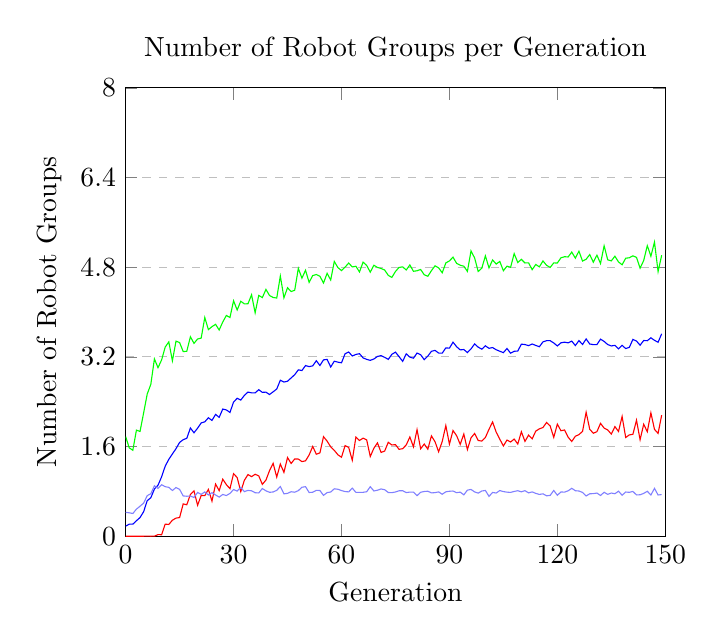
\begin{tikzpicture}
\begin{axis}[
	title={Number of Robot Groups per Generation},
	xlabel={Generation},
	ylabel={Number of Robot Groups},
	xmin=0, xmax=150,
	ymin=0, ymax=8,
	xtick={0.0,30.0,60.0,90.0,120.0,150.0},
	ytick={0.0,1.6,3.2,4.800000000000001,6.4,8.0},
	ymajorgrids=true,
	grid style=dashed,
]

\addplot[
	color=green,
	]
	coordinates {
	(0,1.7779166666666668)(1,1.5761111111111115)(2,1.533888888888889)(3,1.8926388888888888)(4,1.8686111111111112)(5,2.2)(6,2.5370833333333334)(7,2.7093055555555554)(8,3.16375)(9,3.0069444444444438)(10,3.1451388888888894)(11,3.375555555555555)(12,3.467361111111112)(13,3.129861111111111)(14,3.480694444444444)(15,3.4552777777777774)(16,3.294305555555555)(17,3.3)(18,3.5588888888888888)(19,3.441527777777778)(20,3.518472222222223)(21,3.535138888888889)(22,3.9024999999999994)(23,3.686388888888889)(24,3.7391666666666663)(25,3.7808333333333333)(26,3.679027777777778)(27,3.8230555555555554)(28,3.938194444444444)(29,3.902638888888889)(30,4.20125)(31,4.03625)(32,4.192083333333334)(33,4.146249999999999)(34,4.147222222222223)(35,4.307638888888889)(36,3.987083333333333)(37,4.296944444444445)(38,4.258333333333334)(39,4.403472222222223)(40,4.2948611111111115)(41,4.259861111111111)(42,4.249722222222223)(43,4.642916666666666)(44,4.254444444444445)(45,4.43375)(46,4.365277777777778)(47,4.388750000000001)(48,4.779305555555555)(49,4.604166666666667)(50,4.745277777777777)(51,4.529861111111111)(52,4.650972222222222)(53,4.6691666666666665)(54,4.638472222222222)(55,4.517222222222222)(56,4.690694444444444)(57,4.571944444444444)(58,4.902222222222222)(59,4.794305555555556)(60,4.739583333333334)(61,4.801527777777777)(62,4.874305555555556)(63,4.805)(64,4.816666666666666)(65,4.715416666666666)(66,4.890555555555555)(67,4.832222222222223)(68,4.711805555555555)(69,4.834722222222222)(70,4.795833333333333)(71,4.777500000000001)(72,4.749722222222222)(73,4.654305555555555)(74,4.618333333333334)(75,4.723194444444444)(76,4.79625)(77,4.805833333333333)(78,4.750555555555556)(79,4.840277777777778)(80,4.727083333333334)(81,4.736805555555556)(82,4.759166666666666)(83,4.665416666666666)(84,4.638055555555555)(85,4.738194444444445)(86,4.825)(87,4.788333333333333)(88,4.7)(89,4.87611111111111)(90,4.9125000000000005)(91,4.9793055555555545)(92,4.868611111111112)(93,4.835138888888888)(94,4.818055555555555)(95,4.725555555555556)(96,5.0905555555555555)(97,4.965972222222222)(98,4.723333333333333)(99,4.782361111111111)(100,5.0025)(101,4.7868055555555555)(102,4.929861111111111)(103,4.856111111111112)(104,4.903055555555556)(105,4.736805555555556)(106,4.81875)(107,4.797499999999999)(108,5.042638888888889)(109,4.884027777777778)(110,4.940138888888889)(111,4.8758333333333335)(112,4.878055555555556)(113,4.755833333333334)(114,4.848333333333334)(115,4.805833333333333)(116,4.911944444444445)(117,4.83375)(118,4.796666666666667)(119,4.876527777777778)(120,4.874583333333334)(121,4.967638888888889)(122,4.987222222222222)(123,4.9825)(124,5.069722222222223)(125,4.961388888888889)(126,5.085833333333333)(127,4.908888888888889)(128,4.941944444444445)(129,5.025416666666666)(130,4.8886111111111115)(131,5.015)(132,4.865972222222223)(133,5.182222222222222)(134,4.931805555555556)(135,4.912916666666667)(136,4.9961111111111105)(137,4.894027777777778)(138,4.843333333333334)(139,4.960416666666666)(140,4.9686111111111115)(141,5.002638888888889)(142,4.975416666666667)(143,4.782777777777778)(144,4.919444444444444)(145,5.184444444444445)(146,4.994861111111112)(147,5.2484722222222215)(148,4.721805555555556)(149,5.0136111111111115)
	};
\addplot[
	color=blue,
	]
	coordinates {
	(0,0.1786111111111111)(1,0.21471064814814816)(2,0.2146585648148148)(3,0.2760416666666667)(4,0.3327604166666667)(5,0.43712962962962965)(6,0.6337905092592592)(7,0.6861400462962962)(8,0.8412673611111111)(9,0.9099131944444445)(10,1.0595543981481481)(11,1.2499305555555555)(12,1.3720370370370372)(13,1.4673958333333335)(14,1.56203125)(15,1.6729224537037037)(16,1.7222395833333333)(17,1.7467071759259258)(18,1.9304108796296293)(19,1.8457349537037038)(20,1.9270081018518517)(21,2.0214699074074076)(22,2.040601851851852)(23,2.1136863425925934)(24,2.065659722222222)(25,2.1735011574074075)(26,2.1209375)(27,2.269265046296296)(28,2.253333333333333)(29,2.2084837962962967)(30,2.393234953703703)(31,2.460775462962963)(32,2.428298611111111)(33,2.5127256944444443)(34,2.571545138888889)(35,2.5580381944444444)(36,2.557905092592593)(37,2.614265046296296)(38,2.566875)(39,2.5705092592592598)(40,2.527945601851852)(41,2.5764351851851854)(42,2.626140046296296)(43,2.7829976851851854)(44,2.750364583333333)(45,2.765613425925926)(46,2.8238425925925927)(47,2.8827719907407405)(48,2.9686979166666667)(49,2.9564467592592596)(50,3.0448206018518515)(51,3.0258912037037042)(52,3.039415509259259)(53,3.1308217592592595)(54,3.045763888888889)(55,3.146383101851852)(56,3.155121527777778)(57,3.019346064814815)(58,3.1225520833333333)(59,3.105538194444445)(60,3.0941782407407405)(61,3.255995370370371)(62,3.286863425925926)(63,3.2152199074074077)(64,3.243321759259259)(65,3.2569849537037037)(66,3.181435185185185)(67,3.1557291666666667)(68,3.1374421296296293)(69,3.1623437500000002)(70,3.2077662037037036)(71,3.2224363425925926)(72,3.1918692129629624)(73,3.1549826388888893)(74,3.2454745370370373)(75,3.2846643518518515)(76,3.204340277777778)(77,3.1201851851851847)(78,3.2545081018518514)(79,3.1958912037037033)(80,3.1762557870370367)(81,3.2682754629629636)(82,3.2382870370370376)(83,3.1497627314814816)(84,3.213506944444444)(85,3.2994155092592585)(86,3.3161458333333336)(87,3.267390046296296)(88,3.2662037037037033)(89,3.3599247685185185)(90,3.355596064814814)(91,3.4622627314814816)(92,3.381221064814815)(93,3.3247743055555556)(94,3.3311979166666665)(95,3.2768865740740742)(96,3.3418807870370375)(97,3.4312152777777776)(98,3.3730324074074076)(99,3.337384259259259)(100,3.39675925925926)(101,3.3530613425925915)(102,3.36615162037037)(103,3.3271238425925924)(104,3.3006307870370373)(105,3.275306712962963)(106,3.34927662037037)(107,3.2654861111111106)(108,3.299762731481482)(109,3.3043865740740745)(110,3.426909722222222)(111,3.420387731481481)(112,3.3998148148148144)(113,3.4300925925925925)(114,3.4038541666666666)(115,3.3810648148148146)(116,3.4678182870370367)(117,3.4892476851851852)(118,3.488744212962963)(119,3.4480381944444445)(120,3.394398148148148)(121,3.4507407407407404)(122,3.4624537037037038)(123,3.4501273148148153)(124,3.4810185185185185)(125,3.4018634259259257)(126,3.4902025462962962)(127,3.420827546296296)(128,3.5199826388888886)(129,3.4298611111111104)(130,3.418234953703703)(131,3.4194039351851853)(132,3.5162847222222227)(133,3.4754108796296297)(134,3.4200520833333337)(135,3.394490740740741)(136,3.4054340277777784)(137,3.3440046296296293)(138,3.4051620370370372)(139,3.347997685185185)(140,3.369126157407407)(141,3.5115625)(142,3.4824884259259257)(143,3.4073900462962965)(144,3.491903935185185)(145,3.488420138888889)(146,3.5398032407407407)(147,3.495700231481482)(148,3.460167824074074)(149,3.612262731481482)
	};
\addplot[
	color=red,
	]
	coordinates {
	(0,0.0)(1,0.0)(2,0.0)(3,0.0)(4,0.0)(5,0.0)(6,0.0002777777777777778)(7,0.0)(8,0.0001388888888888889)(9,0.028888888888888888)(10,0.025555555555555557)(11,0.21541666666666667)(12,0.20944444444444446)(13,0.2851388888888889)(14,0.32291666666666663)(15,0.3327777777777778)(16,0.5768055555555556)(17,0.5608333333333333)(18,0.7447222222222222)(19,0.808888888888889)(20,0.5515277777777778)(21,0.7268055555555556)(22,0.7237499999999999)(23,0.835138888888889)(24,0.6255555555555555)(25,0.93)(26,0.8127777777777779)(27,1.0174999999999998)(28,0.9193055555555556)(29,0.8484722222222222)(30,1.11625)(31,1.0472222222222223)(32,0.7970833333333331)(33,0.9968055555555555)(34,1.0995833333333331)(35,1.062916666666667)(36,1.1044444444444446)(37,1.0768055555555556)(38,0.924861111111111)(39,1.0013888888888887)(40,1.1706944444444445)(41,1.3004166666666666)(42,1.0549999999999997)(43,1.2876388888888888)(44,1.1388888888888888)(45,1.4034722222222222)(46,1.2979166666666666)(47,1.3784722222222223)(48,1.3763888888888889)(49,1.3312500000000003)(50,1.3444444444444443)(51,1.44875)(52,1.6012499999999998)(53,1.4629166666666664)(54,1.486388888888889)(55,1.775972222222222)(56,1.6965277777777779)(57,1.5941666666666665)(58,1.5313888888888891)(59,1.4531944444444447)(60,1.4093055555555554)(61,1.6159722222222221)(62,1.5833333333333333)(63,1.355138888888889)(64,1.767777777777778)(65,1.7077777777777778)(66,1.7494444444444446)(67,1.718611111111111)(68,1.4218055555555553)(69,1.5697222222222222)(70,1.6655555555555557)(71,1.494722222222222)(72,1.5190277777777779)(73,1.6755555555555555)(74,1.6280555555555556)(75,1.6334722222222222)(76,1.5502777777777779)(77,1.5615277777777776)(78,1.6283333333333332)(79,1.7705555555555554)(80,1.5956944444444445)(81,1.9015277777777777)(82,1.5597222222222225)(83,1.6443055555555555)(84,1.5526388888888891)(85,1.79)(86,1.6852777777777779)(87,1.5063888888888888)(88,1.6904166666666667)(89,1.9741666666666664)(90,1.6419444444444447)(91,1.8856944444444443)(92,1.79375)(93,1.6391666666666667)(94,1.8227777777777778)(95,1.5459722222222223)(96,1.7543055555555558)(97,1.8331944444444443)(98,1.70875)(99,1.6965277777777779)(100,1.7616666666666667)(101,1.9077777777777778)(102,2.037777777777778)(103,1.8568055555555554)(104,1.7309722222222226)(105,1.6097222222222218)(106,1.7159722222222225)(107,1.6808333333333334)(108,1.733472222222222)(109,1.6445833333333335)(110,1.8634722222222222)(111,1.692222222222222)(112,1.8038888888888887)(113,1.7368055555555557)(114,1.8754166666666667)(115,1.9154166666666668)(116,1.9391666666666665)(117,2.029027777777778)(118,1.9681944444444444)(119,1.763472222222222)(120,1.9995833333333333)(121,1.8818055555555557)(122,1.8955555555555557)(123,1.7663888888888888)(124,1.6906944444444443)(125,1.7830555555555556)(126,1.8130555555555554)(127,1.8693055555555553)(128,2.2120833333333336)(129,1.9080555555555556)(130,1.8370833333333332)(131,1.8651388888888885)(132,2.0136111111111115)(133,1.9295833333333334)(134,1.8955555555555552)(135,1.8225)(136,1.9549999999999998)(137,1.8693055555555558)(138,2.1368055555555556)(139,1.7608333333333333)(140,1.807361111111111)(141,1.8177777777777777)(142,2.0702777777777777)(143,1.7209722222222221)(144,1.9980555555555557)(145,1.8643055555555552)(146,2.2018055555555556)(147,1.9059722222222222)(148,1.8344444444444445)(149,2.160833333333333)
	};
\addplot[
	color=blue!50,
	]
	coordinates {
	(0,0.4254617253180636)(1,0.4176927084336511)(2,0.40501904130161087)(3,0.4829067528411115)(4,0.5352951832189629)(5,0.5892953301144767)(6,0.723123831211393)(7,0.7577340995067093)(8,0.8996168671326666)(9,0.8529975186952822)(10,0.9186855135387249)(11,0.8837937560511094)(12,0.8712253248759014)(13,0.8150619063555793)(14,0.8688682345040654)(15,0.8360751669519288)(16,0.7183544492237468)(17,0.7133962906922541)(18,0.7163063949131715)(19,0.691481181571373)(20,0.7804496986780911)(21,0.7465414509329554)(22,0.7903898560669896)(23,0.7346144617481453)(24,0.7764220759461136)(25,0.7355756381848465)(26,0.6978357859639142)(27,0.7444747885674556)(28,0.726044235861343)(29,0.7635145190204099)(30,0.8325589668586407)(31,0.8050398574006596)(32,0.8712898126212465)(33,0.7950787339665032)(34,0.8172408502726076)(35,0.8101002593293523)(36,0.7757247387913577)(37,0.7718650770792915)(38,0.8507111866597911)(39,0.8098125421028177)(40,0.7830137856139192)(41,0.7892442618155032)(42,0.8185616607859145)(43,0.8865887257500167)(44,0.7551514762887303)(45,0.7646796240643006)(46,0.7936065022275041)(47,0.7847640530678643)(48,0.813030163371307)(49,0.872884580872227)(50,0.8844635516856482)(51,0.7797194511169342)(52,0.7841055144775674)(53,0.8185973792447001)(54,0.8150750695764195)(55,0.7285026606390939)(56,0.7779666182465569)(57,0.7882647118834315)(58,0.8458833293238887)(59,0.8377974062228614)(60,0.8144963758456041)(61,0.7963096373758011)(62,0.791093941306781)(63,0.8581679655670745)(64,0.7828541444790397)(65,0.7828458172826736)(66,0.782886945718661)(67,0.7932976004137109)(68,0.8835559445611382)(69,0.8069793293496375)(70,0.8209068835022523)(71,0.8427358428540649)(72,0.8295470236010242)(73,0.7796664587245896)(74,0.776703403532636)(75,0.789011663763685)(76,0.8099188715706771)(77,0.8121852745091785)(78,0.7780148586006894)(79,0.7868172926987632)(80,0.7868004918296662)(81,0.7234232993142145)(82,0.7834421279110473)(83,0.7981222339070412)(84,0.8024884663216237)(85,0.772975599642592)(86,0.7774185122815578)(87,0.7904214525938853)(88,0.7487060028153566)(89,0.7919387064534106)(90,0.8019191869954936)(91,0.8060039401430051)(92,0.7765098003768298)(93,0.786073870699236)(94,0.7377787665310044)(95,0.8218769133301215)(96,0.834676224496771)(97,0.7895689356201571)(98,0.7681492475307492)(99,0.8064767897911796)(100,0.8162174787069509)(101,0.710533953249728)(102,0.7813419125722441)(103,0.7704325816277484)(104,0.814556882465565)(105,0.7960607437991221)(106,0.7860069801559195)(107,0.7814020839525442)(108,0.7989661868614408)(109,0.8112471023205837)(110,0.7919731372531148)(111,0.8123781094711314)(112,0.7725256992869874)(113,0.7905131593828729)(114,0.7641759885981425)(115,0.7448714919941677)(116,0.7561728186058629)(117,0.7208262974235952)(118,0.7280641150194364)(119,0.8161199878330427)(120,0.7308323802940503)(121,0.7890861687112545)(122,0.7865658195667969)(123,0.8106167749911858)(124,0.8541720034943239)(125,0.8117559179800965)(126,0.8061810322291417)(127,0.7808985748826995)(128,0.7183230295331609)(129,0.7565254497718875)(130,0.7600800396099365)(131,0.7696983965483409)(132,0.726427918699271)(133,0.7838349634202023)(134,0.7468408759504754)(135,0.769993120894664)(136,0.7576945264703074)(137,0.8029402429619794)(138,0.7306241643584157)(139,0.7885306588168193)(140,0.7826085242051224)(141,0.7984683196777242)(142,0.7362239164343475)(143,0.7395304062888189)(144,0.7637361643728297)(145,0.8014718205859099)(146,0.735241911038397)(147,0.8529661273732119)(148,0.7353072733795413)(149,0.7429127089203906)
	};
\end{axis}
\end{tikzpicture}
}
		\caption{Some sample caption}
		\label{fig:number-of-groups-easy}
	\end{subfigure}%
}
\\
\\
\\
\\
	\makebox[\linewidth][c]{%
	\begin{subfigure}[b]{0.7\textwidth}
		\centering
		\resizebox{0.9\linewidth}{!}{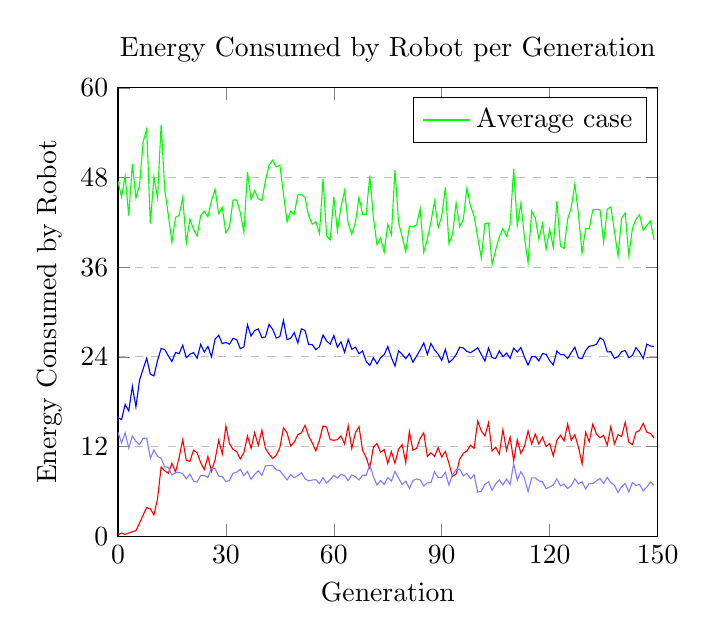
\begin{tikzpicture}
\begin{axis}[
	title={Energy Consumed by Robot per Generation},
	xlabel={Generation},
	ylabel={Energy Consumed by Robot},
	xmin=0, xmax=150,
	ymin=0, ymax=60,
	xtick={0.0,30.0,60.0,90.0,120.0,150.0},
	ytick={0.0,12.0,24.0,36.0,48.0,60.0},
	ymajorgrids=true,
	grid style=dashed,
]

\addplot[
	color=green,
	]
	coordinates {
	(0,47.5)(1,45.416666666666664)(2,48.166666666666664)(3,42.916666666666664)(4,49.833333333333336)(5,45.25)(6,47.00000000000001)(7,52.75)(8,54.50000000000001)(9,41.833333333333336)(10,48.083333333333336)(11,45.33333333333333)(12,55.083333333333336)(13,46.41666666666667)(14,43.0)(15,39.333333333333336)(16,42.666666666666664)(17,42.916666666666664)(18,45.333333333333336)(19,39.25)(20,42.41666666666667)(21,41.08333333333333)(22,40.166666666666664)(23,42.91666666666667)(24,43.5)(25,42.75)(26,44.916666666666664)(27,46.41666666666667)(28,43.16666666666667)(29,44.0)(30,40.583333333333336)(31,41.41666666666667)(32,44.99999999999999)(33,44.99999999999999)(34,43.333333333333336)(35,40.666666666666664)(36,48.75)(37,45.083333333333336)(38,46.25000000000001)(39,45.16666666666667)(40,44.91666666666667)(41,47.583333333333336)(42,49.666666666666664)(43,50.333333333333336)(44,49.41666666666667)(45,49.666666666666664)(46,45.83333333333333)(47,42.08333333333333)(48,43.5)(49,43.083333333333336)(50,45.66666666666667)(51,45.75)(52,45.333333333333336)(53,42.916666666666664)(54,41.75000000000001)(55,42.083333333333336)(56,40.5)(57,47.833333333333336)(58,40.16666666666667)(59,39.66666666666667)(60,45.416666666666664)(61,40.833333333333336)(62,44.083333333333336)(63,46.25)(64,41.833333333333336)(65,40.416666666666664)(66,42.0)(67,45.333333333333336)(68,43.08333333333333)(69,43.083333333333336)(70,48.25)(71,42.66666666666667)(72,39.0)(73,39.916666666666664)(74,38.0)(75,41.75)(76,40.333333333333336)(77,49.0)(78,41.99999999999999)(79,40.083333333333336)(80,38.08333333333333)(81,41.49999999999999)(82,41.41666666666667)(83,41.666666666666664)(84,43.83333333333333)(85,38.0)(86,39.75)(87,42.08333333333333)(88,44.833333333333336)(89,41.333333333333336)(90,42.83333333333333)(91,46.666666666666664)(92,39.16666666666667)(93,40.416666666666664)(94,44.583333333333336)(95,41.416666666666664)(96,42.416666666666664)(97,46.58333333333333)(98,44.166666666666664)(99,42.83333333333333)(100,40.0)(101,37.25)(102,41.833333333333336)(103,41.916666666666664)(104,36.333333333333336)(105,38.333333333333336)(106,40.083333333333336)(107,41.16666666666667)(108,40.166666666666664)(109,41.66666666666667)(110,49.166666666666664)(111,41.583333333333336)(112,44.583333333333336)(113,39.916666666666664)(114,36.583333333333336)(115,43.5)(116,42.583333333333336)(117,39.75)(118,41.83333333333333)(119,38.41666666666667)(120,41.08333333333333)(121,38.666666666666664)(122,44.833333333333336)(123,38.83333333333333)(124,38.5)(125,42.41666666666667)(126,44.0)(127,47.166666666666664)(128,43.08333333333333)(129,37.91666666666667)(130,41.166666666666664)(131,41.166666666666664)(132,43.666666666666664)(133,43.75000000000001)(134,43.666666666666664)(135,39.33333333333333)(136,43.75)(137,44.08333333333333)(138,40.833333333333336)(139,37.5)(140,42.583333333333336)(141,43.25)(142,37.583333333333336)(143,41.16666666666667)(144,42.41666666666667)(145,43.0)(146,40.916666666666664)(147,41.58333333333333)(148,42.166666666666664)(149,39.666666666666664)
	};
\addplot[
	color=blue,
	]
	coordinates {
	(0,15.875)(1,15.600694444444445)(2,17.631944444444443)(3,16.767361111111114)(4,20.038194444444446)(5,17.305555555555554)(6,20.87847222222222)(7,22.38888888888889)(8,23.812499999999996)(9,21.684027777777782)(10,21.458333333333336)(11,23.5)(12,25.11111111111111)(13,24.986111111111114)(14,24.128472222222218)(15,23.36805555555555)(16,24.59027777777778)(17,24.430555555555554)(18,25.559027777777782)(19,23.895833333333336)(20,24.34722222222222)(21,24.572916666666668)(22,23.81944444444445)(23,25.677083333333332)(24,24.642361111111114)(25,25.395833333333336)(26,24.0)(27,26.364583333333336)(28,26.892361111111114)(29,25.77430555555556)(30,25.930555555555557)(31,25.70486111111111)(32,26.46527777777778)(33,26.315972222222225)(34,25.093750000000004)(35,25.32638888888889)(36,28.29861111111111)(37,26.791666666666664)(38,27.53472222222222)(39,27.73611111111111)(40,26.569444444444443)(41,26.677083333333332)(42,28.34027777777778)(43,27.680555555555557)(44,26.517361111111114)(45,26.71875)(46,28.874999999999996)(47,26.29861111111111)(48,26.486111111111114)(49,27.239583333333332)(50,25.864583333333336)(51,27.75)(52,27.538194444444443)(53,25.65972222222222)(54,25.624999999999996)(55,24.965277777777775)(56,25.34375)(57,26.923611111111114)(58,26.12152777777778)(59,25.701388888888886)(60,26.850694444444443)(61,25.29513888888889)(62,25.99652777777778)(63,24.60763888888889)(64,26.333333333333332)(65,25.00347222222222)(66,25.305555555555557)(67,24.40972222222222)(68,24.795138888888893)(69,23.392361111111107)(70,22.85416666666667)(71,23.885416666666664)(72,23.069444444444443)(73,23.875)(74,24.302083333333332)(75,25.381944444444446)(76,23.90277777777778)(77,22.770833333333336)(78,24.81597222222222)(79,24.354166666666664)(80,23.756944444444443)(81,24.4375)(82,23.291666666666664)(83,24.100694444444443)(84,24.927083333333332)(85,25.864583333333332)(86,24.315972222222218)(87,25.795138888888893)(88,24.920138888888893)(89,24.364583333333332)(90,23.517361111111114)(91,25.006944444444443)(92,23.23263888888889)(93,23.645833333333336)(94,24.295138888888886)(95,25.302083333333332)(96,25.177083333333332)(97,24.72916666666667)(98,24.555555555555557)(99,24.857638888888886)(100,25.20833333333333)(101,24.32638888888889)(102,23.43402777777778)(103,25.177083333333332)(104,23.87847222222222)(105,23.798611111111114)(106,24.80208333333333)(107,24.017361111111114)(108,24.510416666666668)(109,23.802083333333336)(110,25.163194444444446)(111,24.631944444444446)(112,25.260416666666668)(113,23.947916666666664)(114,22.913194444444446)(115,24.010416666666664)(116,24.045138888888886)(117,23.44097222222222)(118,24.440972222222225)(119,24.354166666666664)(120,23.503472222222225)(121,22.909722222222218)(122,24.784722222222225)(123,24.312499999999996)(124,24.274305555555557)(125,23.770833333333332)(126,24.55902777777778)(127,25.298611111111114)(128,23.864583333333336)(129,23.76041666666667)(130,24.836805555555557)(131,25.43402777777778)(132,25.493055555555554)(133,25.680555555555557)(134,26.53819444444444)(135,26.246527777777775)(136,24.67013888888889)(137,24.680555555555557)(138,23.79861111111111)(139,24.01041666666667)(140,24.71875)(141,24.836805555555557)(142,23.88888888888889)(143,24.1875)(144,25.23611111111111)(145,24.62152777777778)(146,23.781250000000004)(147,25.701388888888893)(148,25.458333333333332)(149,25.368055555555557)
	};
	\addlegendentry{Average case}
\addplot[
	color=red,
	]
	coordinates {
	(0,0.16666666666666666)(1,0.41666666666666663)(2,0.25)(3,0.41666666666666663)(4,0.5833333333333333)(5,0.75)(6,1.75)(7,2.8333333333333335)(8,3.8333333333333335)(9,3.666666666666667)(10,2.833333333333333)(11,5.0)(12,9.25)(13,8.75)(14,8.416666666666666)(15,9.75)(16,8.583333333333334)(17,10.5)(18,12.916666666666666)(19,10.166666666666666)(20,10.0)(21,11.5)(22,11.166666666666666)(23,9.833333333333332)(24,8.916666666666666)(25,10.666666666666668)(26,8.666666666666666)(27,10.25)(28,12.833333333333334)(29,11.0)(30,14.75)(31,12.416666666666668)(32,11.583333333333334)(33,11.333333333333334)(34,10.333333333333332)(35,11.166666666666666)(36,13.416666666666668)(37,11.75)(38,13.833333333333334)(39,12.166666666666666)(40,14.166666666666666)(41,11.75)(42,11.0)(43,10.416666666666666)(44,10.833333333333332)(45,11.833333333333332)(46,14.5)(47,13.833333333333332)(48,12.083333333333332)(49,12.583333333333334)(50,13.583333333333332)(51,13.833333333333334)(52,14.833333333333334)(53,13.416666666666666)(54,12.5)(55,11.416666666666668)(56,12.833333333333334)(57,14.749999999999998)(58,14.583333333333334)(59,12.916666666666668)(60,12.833333333333334)(61,12.916666666666666)(62,13.416666666666668)(63,12.333333333333334)(64,14.749999999999998)(65,11.749999999999998)(66,13.833333333333334)(67,14.666666666666668)(68,11.5)(69,10.5)(70,9.083333333333334)(71,11.916666666666666)(72,12.416666666666668)(73,11.25)(74,11.583333333333334)(75,9.749999999999998)(76,11.333333333333334)(77,9.75)(78,11.666666666666668)(79,12.249999999999998)(80,9.833333333333334)(81,13.999999999999998)(82,11.5)(83,11.749999999999998)(84,13.083333333333332)(85,13.833333333333332)(86,10.666666666666666)(87,11.166666666666666)(88,10.666666666666668)(89,11.833333333333334)(90,10.583333333333332)(91,11.333333333333334)(92,9.75)(93,7.999999999999999)(94,8.333333333333334)(95,10.333333333333332)(96,11.083333333333332)(97,11.416666666666666)(98,12.166666666666666)(99,11.75)(100,15.416666666666668)(101,14.083333333333334)(102,13.416666666666666)(103,15.166666666666666)(104,11.416666666666666)(105,11.916666666666666)(106,11.0)(107,14.249999999999998)(108,11.5)(109,13.250000000000002)(110,10.083333333333334)(111,12.916666666666668)(112,11.083333333333334)(113,12.0)(114,14.083333333333332)(115,12.333333333333334)(116,13.666666666666666)(117,12.333333333333332)(118,13.249999999999998)(119,11.999999999999998)(120,12.416666666666666)(121,10.750000000000002)(122,12.833333333333334)(123,13.500000000000002)(124,12.749999999999998)(125,15.0)(126,12.833333333333334)(127,13.583333333333334)(128,11.916666666666666)(129,9.666666666666666)(130,13.916666666666664)(131,12.666666666666666)(132,15.000000000000002)(133,13.666666666666666)(134,13.166666666666668)(135,13.499999999999998)(136,12.166666666666666)(137,14.666666666666666)(138,12.333333333333334)(139,13.583333333333332)(140,13.333333333333334)(141,15.25)(142,12.583333333333334)(143,12.25)(144,13.916666666666664)(145,14.166666666666666)(146,15.083333333333334)(147,13.916666666666668)(148,13.749999999999998)(149,13.166666666666668)
	};
\addplot[
	color=blue!50,
	]
	coordinates {
	(0,13.90267508831089)(1,12.47226672500314)(2,13.829624590349557)(3,11.789274573223636)(4,13.413844666176374)(5,12.688883505652079)(6,12.257167226349628)(7,13.106379522748576)(8,13.110225882701092)(9,10.426841176890743)(10,11.545012687873774)(11,10.67171785150359)(12,10.424450249766346)(13,9.265681375173264)(14,9.216473419020714)(15,8.18516134471119)(16,8.515399246235402)(17,8.520171334785168)(18,8.384822908560828)(19,7.6774441419309625)(20,8.313776502588945)(21,7.383943844763538)(22,7.226351019568069)(23,8.14228601526083)(24,8.120382544078307)(25,7.864600729350112)(26,9.128590844517353)(27,9.036741475390718)(28,8.037961055029903)(29,7.966856790838541)(30,7.299041024437335)(31,7.464516831172022)(32,8.40847260936773)(33,8.579220170591192)(34,8.958164879835902)(35,8.104103361144595)(36,8.675555453991384)(37,7.604493560433139)(38,8.26013414114198)(39,8.761153843912247)(40,8.139475024194684)(41,9.390051821918272)(42,9.456435175042492)(43,9.467155038754942)(44,8.884298136861146)(45,8.765882660828167)(46,8.160842619939334)(47,7.529402918218205)(48,8.23719682195419)(49,7.829660062721458)(50,8.107746091565126)(51,8.486096268382749)(52,7.703726537669015)(53,7.38905924607209)(54,7.518516882515916)(55,7.5622872574268545)(56,7.0341639126835975)(57,7.826614501890382)(58,7.107693029436927)(59,7.57718604891149)(60,8.133221119978028)(61,7.799516914047528)(62,8.262157162117933)(63,8.112632253380381)(64,7.428536064132439)(65,8.20771428378926)(66,7.964761511693097)(67,7.521830821678718)(68,8.158001693026549)(69,8.160197053607996)(70,9.586478122984042)(71,7.9803460395866885)(72,6.846341369349167)(73,7.444256782802697)(74,6.920720916403518)(75,7.860331642475469)(76,7.366497370163017)(77,8.670466769779681)(78,7.777506107446994)(79,6.903838564445453)(80,7.35614985562651)(81,6.384405180049235)(82,7.4438595473128455)(83,7.671165252945963)(84,7.539413194921626)(85,6.720120552922453)(86,7.130831208411188)(87,7.172999931789191)(88,8.606450347921854)(89,7.857038781391409)(90,7.8778203960473725)(91,8.539956688965365)(92,6.83866536730472)(93,8.22220527383319)(94,8.888584015865774)(95,8.98686113162109)(96,8.070860893944689)(97,8.414012067462812)(98,7.674393348379541)(99,8.202483047272889)(100,5.889440699055045)(101,6.020486835739401)(102,6.936682403265805)(103,7.285110867790616)(104,6.14522944810159)(105,7.002938325618786)(106,7.532862750630825)(107,6.8635942184122065)(108,7.644630681967605)(109,6.897340718388838)(110,9.719004561105358)(111,7.521371653077291)(112,8.646030969845379)(113,7.763144800383364)(114,5.946528149668643)(115,7.806759264864431)(116,7.80524377897229)(117,7.419492711009111)(118,7.285768141969099)(119,6.342404244214291)(120,6.586610616391859)(121,6.848151449808877)(122,7.686711128937212)(123,6.742661657630832)(124,6.940591169370634)(125,6.3826841034697175)(126,6.771104115378577)(127,7.682793579809095)(128,7.003504145793773)(129,7.278668913007887)(130,6.329037875691446)(131,7.066771096257844)(132,7.0322988790245855)(133,7.416565840293636)(134,7.702236216427049)(135,7.05317767586283)(136,7.885177271954002)(137,7.1902223963047796)(138,6.811278373303489)(139,5.8421893515899)(140,6.624523656584128)(141,7.0445051765022)(142,5.916024314177142)(143,7.178376729674846)(144,6.794461522518879)(145,6.921970051556661)(146,6.055792718647465)(147,6.577610085427416)(148,7.244686210467727)(149,6.843831608522187)
	};
\end{axis}
\end{tikzpicture}
}
		\caption{Some sample caption}
		\label{fig:energy-consumed-by-robot-easy}
	\end{subfigure}%
	\begin{subfigure}[b]{0.7\textwidth}
		\centering
		\resizebox{0.9\linewidth}{!}{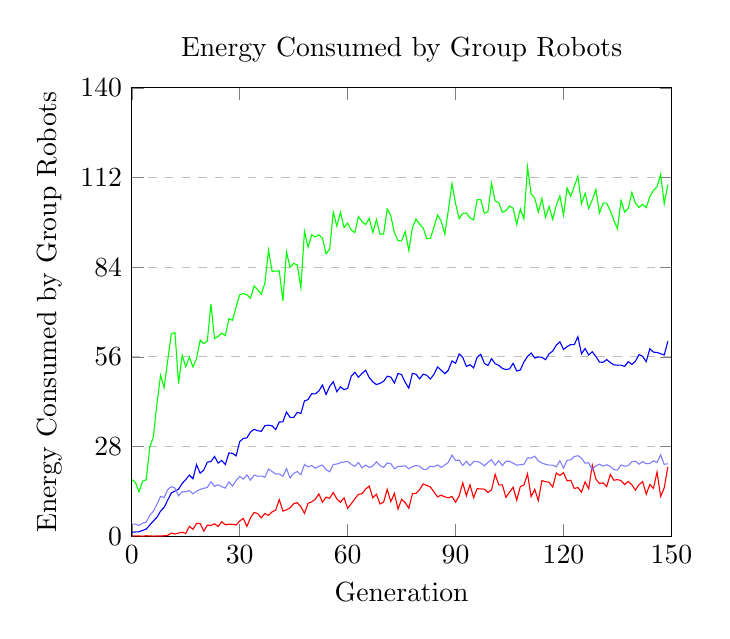
\begin{tikzpicture}
\begin{axis}[
	title={Energy Consumed by Group Robots},
	xlabel={Generation},
	ylabel={Energy Consumed by Group Robots},
	xmin=0, xmax=150,
	ymin=0, ymax=140,
	xtick={0.0,30.0,60.0,90.0,120.0,150.0},
	ytick={0.0,28.0,56.0,84.0,112.0,140.0},
	ymajorgrids=true,
	grid style=dashed,
]

\addplot[
	color=green,
	]
	coordinates {
	(0,17.666666666666664)(1,16.805555555555557)(2,13.861111111111109)(3,17.194444444444446)(4,17.583333333333332)(5,27.72222222222222)(6,31.055555555555554)(7,41.49999999999999)(8,50.222222222222214)(9,46.416666666666664)(10,54.972222222222214)(11,63.19444444444444)(12,63.55555555555555)(13,47.69444444444445)(14,56.55555555555556)(15,52.888888888888886)(16,55.972222222222214)(17,52.833333333333336)(18,55.49999999999999)(19,61.22222222222223)(20,60.111111111111114)(21,60.97222222222222)(22,72.55555555555554)(23,61.72222222222222)(24,62.388888888888886)(25,63.361111111111114)(26,62.61111111111111)(27,67.91666666666667)(28,67.41666666666666)(29,71.6111111111111)(30,75.3888888888889)(31,75.77777777777777)(32,75.38888888888889)(33,74.33333333333334)(34,78.16666666666666)(35,76.94444444444444)(36,75.58333333333334)(37,78.99999999999999)(38,89.38888888888889)(39,82.69444444444444)(40,82.77777777777779)(41,82.83333333333333)(42,73.47222222222221)(43,88.75)(44,83.94444444444444)(45,85.19444444444446)(46,84.69444444444443)(47,77.52777777777777)(48,95.16666666666667)(49,90.25)(50,94.13888888888887)(51,93.47222222222223)(52,94.11111111111111)(53,93.02777777777777)(54,88.19444444444443)(55,89.61111111111113)(56,101.22222222222223)(57,96.80555555555556)(58,101.11111111111113)(59,96.38888888888887)(60,97.77777777777779)(61,95.58333333333334)(62,94.80555555555554)(63,99.80555555555554)(64,98.27777777777777)(65,97.30555555555556)(66,99.25000000000001)(67,94.83333333333333)(68,98.88888888888889)(69,94.27777777777777)(70,94.38888888888891)(71,102.19444444444444)(72,100.05555555555556)(73,94.69444444444443)(74,92.27777777777779)(75,92.19444444444444)(76,95.11111111111113)(77,89.19444444444446)(78,96.30555555555556)(79,99.00000000000001)(80,97.41666666666666)(81,96.2222222222222)(82,92.88888888888887)(83,93.0)(84,96.5)(85,100.30555555555556)(86,98.41666666666666)(87,94.30555555555554)(88,101.83333333333333)(89,110.08333333333331)(90,103.8888888888889)(91,99.16666666666666)(92,100.75000000000001)(93,100.94444444444447)(94,99.38888888888889)(95,98.74999999999999)(96,105.11111111111111)(97,105.1111111111111)(98,100.83333333333334)(99,101.3611111111111)(100,110.19444444444443)(101,104.72222222222221)(102,104.16666666666667)(103,101.16666666666666)(104,101.6388888888889)(105,103.11111111111111)(106,102.44444444444444)(107,97.41666666666667)(108,102.16666666666667)(109,99.08333333333334)(110,115.30555555555556)(111,106.86111111111113)(112,105.61111111111111)(113,101.16666666666664)(114,105.41666666666667)(115,99.55555555555556)(116,102.94444444444444)(117,98.94444444444443)(118,103.3888888888889)(119,106.27777777777779)(120,100.22222222222221)(121,108.75)(122,106.13888888888889)(123,109.25)(124,112.3888888888889)(125,103.74999999999999)(126,107.08333333333333)(127,102.3888888888889)(128,105.05555555555556)(129,108.30555555555554)(130,100.91666666666667)(131,103.99999999999999)(132,104.0)(133,101.61111111111111)(134,98.61111111111109)(135,96.02777777777779)(136,104.88888888888887)(137,101.19444444444443)(138,102.36111111111111)(139,107.30555555555553)(140,103.9722222222222)(141,102.69444444444444)(142,103.63888888888889)(143,102.58333333333334)(144,106.05555555555554)(145,107.99999999999999)(146,109.08333333333333)(147,113.02777777777776)(148,103.80555555555557)(149,109.77777777777779)
	};
\addplot[
	color=blue,
	]
	coordinates {
	(0,1.204861111111111)(1,1.3310185185185184)(2,1.378472222222222)(3,1.804398148148148)(4,2.204861111111112)(5,3.4837962962962967)(6,4.756944444444445)(7,5.918981481481482)(8,7.8402777777777795)(9,9.03125)(10,11.315972222222223)(11,13.51273148148148)(12,14.090277777777779)(13,14.658564814814815)(14,16.48611111111111)(15,17.672453703703706)(16,19.08101851851852)(17,17.960648148148145)(18,22.34027777777778)(19,19.663194444444446)(20,20.63888888888889)(21,23.10416666666667)(22,23.297453703703706)(23,24.890046296296294)(24,22.835648148148152)(25,23.644675925925924)(26,22.37615740740741)(27,25.99652777777778)(28,25.868055555555554)(29,25.077546296296294)(30,29.55439814814815)(31,30.521990740740744)(32,30.71412037037037)(33,32.55324074074074)(34,33.363425925925924)(35,32.949074074074076)(36,32.7349537037037)(37,34.520833333333336)(38,34.68287037037037)(39,34.45370370370371)(40,33.32175925925926)(41,35.64699074074074)(42,35.71527777777778)(43,38.78935185185185)(44,37.10300925925927)(45,37.1099537037037)(46,38.645833333333336)(47,38.33101851851852)(48,42.25000000000001)(49,42.65740740740741)(50,44.482638888888886)(51,44.447916666666664)(52,45.34606481481481)(53,47.214120370370374)(54,44.24189814814814)(55,46.739583333333336)(56,48.23148148148148)(57,45.12847222222222)(58,46.646990740740755)(59,45.75810185185185)(60,46.15625)(61,49.954861111111114)(62,51.19444444444445)(63,49.61689814814814)(64,50.81944444444444)(65,51.81944444444444)(66,49.55671296296297)(67,48.186342592592595)(68,47.34837962962963)(69,47.741898148148145)(70,48.351851851851855)(71,49.954861111111114)(72,49.682870370370374)(73,47.8125)(74,50.79398148148147)(75,50.451388888888886)(76,48.05902777777777)(77,46.22222222222223)(78,50.84606481481481)(79,50.58796296296296)(80,49.10532407407407)(81,50.60069444444444)(82,50.2361111111111)(83,49.101851851851855)(84,50.563657407407405)(85,52.86574074074075)(86,51.83912037037037)(87,50.74768518518519)(88,51.863425925925924)(89,54.730324074074076)(90,53.97800925925925)(91,56.90393518518519)(92,55.85416666666667)(93,52.98495370370371)(94,53.53819444444444)(95,52.56018518518518)(96,55.87731481481482)(97,56.79513888888888)(98,53.95949074074074)(99,53.29629629629629)(100,55.44907407407408)(101,53.8599537037037)(102,53.36805555555556)(103,52.383101851851855)(104,52.04050925925925)(105,52.24884259259259)(106,53.97569444444444)(107,51.57754629629629)(108,51.91203703703703)(109,54.4212962962963)(110,56.13773148148148)(111,57.211805555555564)(112,55.63773148148149)(113,55.97222222222223)(114,55.864583333333336)(115,55.12268518518518)(116,56.9699074074074)(117,57.80439814814815)(118,59.67476851851852)(119,60.68055555555556)(120,58.32175925925926)(121,59.19907407407407)(122,59.83564814814815)(123,59.8425925925926)(124,62.28356481481481)(125,56.949074074074076)(126,58.60416666666666)(127,56.5787037037037)(128,57.599537037037045)(129,56.1087962962963)(130,54.38310185185185)(131,54.28356481481482)(132,55.164351851851855)(133,54.208333333333336)(134,53.51273148148148)(135,53.39467592592593)(136,53.41782407407407)(137,53.00694444444445)(138,54.50462962962962)(139,53.63425925925926)(140,54.644675925925924)(141,56.69560185185185)(142,56.158564814814824)(143,54.5173611111111)(144,58.54050925925927)(145,57.48263888888889)(146,57.375)(147,56.98148148148148)(148,56.581018518518526)(149,60.862268518518526)
	};
\addplot[
	color=red,
	]
	coordinates {
	(0,0.027777777777777776)(1,0.1111111111111111)(2,0.08333333333333333)(3,0.0)(4,0.1388888888888889)(5,0.08333333333333333)(6,0.027777777777777776)(7,0.08333333333333333)(8,0.05555555555555555)(9,0.1388888888888889)(10,0.25)(11,1.0)(12,0.6666666666666667)(13,0.9722222222222222)(14,1.222222222222222)(15,0.888888888888889)(16,3.083333333333333)(17,2.166666666666666)(18,4.0)(19,3.9722222222222214)(20,1.6111111111111112)(21,3.4166666666666665)(22,3.3888888888888884)(23,3.861111111111111)(24,3.0277777777777777)(25,4.5)(26,3.5277777777777777)(27,3.75)(28,3.7222222222222223)(29,3.472222222222222)(30,4.75)(31,5.555555555555555)(32,3.055555555555556)(33,5.777777777777778)(34,7.416666666666667)(35,7.083333333333334)(36,5.722222222222221)(37,7.083333333333333)(38,6.5)(39,7.583333333333332)(40,8.138888888888888)(41,11.416666666666666)(42,7.833333333333334)(43,8.25)(44,8.833333333333332)(45,10.166666666666668)(46,10.444444444444445)(47,9.222222222222221)(48,7.111111111111112)(49,10.277777777777779)(50,10.722222222222221)(51,11.555555555555557)(52,13.194444444444443)(53,10.611111111111112)(54,12.194444444444445)(55,11.833333333333336)(56,13.63888888888889)(57,11.61111111111111)(58,10.583333333333332)(59,11.972222222222221)(60,8.694444444444446)(61,10.13888888888889)(62,11.63888888888889)(63,13.083333333333332)(64,13.277777777777779)(65,14.722222222222221)(66,15.63888888888889)(67,12.0)(68,13.111111111111109)(69,10.055555555555554)(70,10.63888888888889)(71,14.63888888888889)(72,10.777777777777777)(73,13.361111111111112)(74,8.472222222222223)(75,11.527777777777779)(76,10.472222222222223)(77,8.722222222222223)(78,13.277777777777777)(79,13.36111111111111)(80,14.527777777777777)(81,16.333333333333332)(82,15.861111111111109)(83,15.361111111111112)(84,13.805555555555557)(85,12.277777777777779)(86,12.805555555555554)(87,12.277777777777779)(88,12.0)(89,12.416666666666668)(90,10.61111111111111)(91,12.63888888888889)(92,16.66666666666667)(93,12.638888888888891)(94,16.083333333333336)(95,11.999999999999998)(96,14.861111111111109)(97,14.750000000000002)(98,14.694444444444446)(99,13.666666666666666)(100,14.444444444444443)(101,19.305555555555557)(102,16.055555555555557)(103,16.0)(104,12.111111111111109)(105,13.777777777777777)(106,15.277777777777777)(107,11.222222222222223)(108,15.500000000000002)(109,15.972222222222221)(110,19.472222222222225)(111,12.333333333333332)(112,14.63888888888889)(113,11.11111111111111)(114,17.36111111111111)(115,17.02777777777778)(116,16.833333333333336)(117,15.333333333333332)(118,19.75)(119,18.97222222222223)(120,19.833333333333332)(121,17.277777777777775)(122,17.472222222222225)(123,14.888888888888891)(124,15.194444444444443)(125,13.75)(126,16.97222222222222)(127,14.805555555555555)(128,22.194444444444443)(129,17.833333333333332)(130,16.444444444444446)(131,16.666666666666668)(132,15.472222222222221)(133,19.277777777777775)(134,17.47222222222222)(135,17.666666666666664)(136,17.36111111111111)(137,16.13888888888889)(138,17.11111111111111)(139,16.055555555555554)(140,14.388888888888888)(141,16.11111111111111)(142,17.055555555555554)(143,13.111111111111112)(144,16.13888888888889)(145,14.944444444444445)(146,20.02777777777778)(147,12.416666666666668)(148,15.111111111111114)(149,21.611111111111114)
	};
\addplot[
	color=blue!50,
	]
	coordinates {
	(0,3.793637938766837)(1,3.7523379573637192)(2,3.328567501675064)(3,4.030622213270808)(4,4.4200511181489555)(5,6.519824814561398)(6,7.802042272417542)(7,10.02441977439477)(8,12.394071449676321)(9,12.103048049487064)(10,14.57959618435815)(11,15.485529877572361)(12,15.034668068213444)(13,12.603791535892713)(14,13.859131958019335)(15,13.893695320975688)(16,14.276972976489066)(17,13.22815768166678)(18,14.055143819485444)(19,14.622606430366234)(20,14.957302266366)(21,15.235080611643786)(22,17.010023256091696)(23,15.54041286278934)(24,16.06585257567348)(25,15.463743324103445)(26,15.017060927033821)(27,16.99920117965988)(28,15.638964693265052)(29,17.357328711496155)(30,18.65930225851148)(31,17.817017139874075)(32,19.15098610194967)(33,17.49211868808712)(34,19.07601101744591)(35,18.72609079639066)(36,18.781965227909247)(37,18.39148958131118)(38,20.990059804215992)(39,20.19393388085553)(40,19.42155311976079)(41,19.466427884989365)(42,18.674249766031945)(43,21.099624848741005)(44,18.18430051809181)(45,19.639222180868042)(46,20.186544048266615)(47,19.165787771049892)(48,22.406292112976733)(49,21.637076798051105)(50,22.07681205051556)(51,21.19582457976546)(52,21.81479580683102)(53,22.21874003690169)(54,20.751469937438127)(55,20.119478712936015)(56,22.390235817320768)(57,22.532265685785312)(58,22.94179252512627)(59,23.17790456840255)(60,23.374023837530512)(61,22.44264885088899)(62,21.797006412357266)(63,23.033471985534707)(64,21.33204072423209)(65,22.225328737529967)(66,21.463398849893995)(67,21.876051654403554)(68,23.254525487465227)(69,22.04178875176993)(70,21.486804029634754)(71,22.87804553388826)(72,22.6268344731064)(73,21.06987673238088)(74,21.77638873835049)(75,21.843403947318553)(76,21.99489900246392)(77,21.061199648796194)(78,21.733479954188343)(79,22.04848039440876)(80,21.860752690829468)(81,20.872231866412836)(82,20.87737121227454)(83,21.87810009551734)(84,21.649128015090245)(85,22.255461017226825)(86,21.481186985707282)(87,22.229964783114706)(88,23.019410518842715)(89,25.320192971512302)(90,23.640904586511194)(91,23.751498134614707)(92,22.074041947008315)(93,23.40618453196275)(94,22.06262937619204)(95,23.30364861466495)(96,23.367568507380653)(97,22.88888347001476)(98,21.9613032214439)(99,23.05656757258113)(100,23.8795828518469)(101,22.173941163138757)(102,23.555090297325638)(103,22.042569989096897)(104,23.387709176985048)(105,23.408034199414868)(106,22.822599314642197)(107,22.188003546626796)(108,22.318822499079342)(109,22.44671611165769)(110,24.41890101869657)(111,24.42938748046953)(112,24.995956868444676)(113,23.52914829444043)(114,22.84338416929849)(115,22.457801784008492)(116,22.17880289408619)(117,22.1752024655541)(118,21.66844593658571)(119,23.544065436336)(120,21.293477236817772)(121,23.699115144118934)(122,23.858499913315633)(123,24.876558087166273)(124,25.139259805821098)(125,24.370286751592847)(126,22.796628936785954)(127,22.945130761542615)(128,20.712334622816293)(129,22.02718560513645)(130,22.48307169661878)(131,21.892344889711108)(132,22.302944315019634)(133,21.785769583376787)(134,20.78000456681748)(135,20.681228909177996)(136,22.2383585400881)(137,21.85109005991582)(138,22.02406005363854)(139,23.27594489367388)(140,23.413843949583757)(141,22.489554217561924)(142,23.281602832734492)(143,22.636691631241852)(144,22.71564516555098)(145,23.537547512483464)(146,23.02467193574319)(147,25.40396907333671)(148,22.4235322956733)(149,22.629412830065373)
	};
\end{axis}
\end{tikzpicture}
}
		\caption{Some sample caption}
		\label{fig:energy-consumed-by-group-easy}
	\end{subfigure}%

}
\caption{Figure shows results from a simulation in the easy environment (p.2)}
\end{figure}
